% Title page
\frame[plain]{\titlepage}

% Lesson 1. Introduction, main terms and simple examples
\lecture{Intro}{intro}

\section{Course work and grading policy}

\section{Tools and resources}

\begin{frame}
	\frametitle{\insertsection}
	We are going to use SWI-Prolog~--- a comprehensive free Prolog environment.
	\begin{itemize}
		\item You can download SWI-Prolog at this page: \href{https://www.swi-prolog.org/download/stable}{https://www.swi-prolog.org/download/stable}
		\item Complete manual is available at \href{https://www.swi-prolog.org/pldoc/doc_for?object=manual}{https://www.swi-prolog.org/pldoc/doc\_for?object=manual}
		\item Online tool SWISH: \href{https://swish.swi-prolog.org/}{https://swish.swi-prolog.org/}
		\item \textcolor{gray}{Eclipse PDT~--- Prolog Development Tool:} \href{https://sewiki.iai.uni-bonn.de/research/pdt/docs/start}{https://sewiki.iai.uni-bonn.de/research/pdt/docs/start}
		\item Slides will be published weekly in the Google Classroom and on github: \href{https://github.com/Inscriptor/IntroductionToAI}{https://github.com/Inscriptor/IntroductionToAI}
	\end{itemize}
\end{frame}


\section{Work and grading policy}

\begin{frame}
	\frametitle{\insertsection}
	
	\textbf{100\% = 375 points}
	
	\begin{itemize}
		\item 6 Assignments: 5\% + 6\% + 2 x 12\% + 2 x 20\%: 75\%
		\item Exam: 40\%
		\begin{itemize}
			\item 5 = 150 pts, 4 = 100 pts, 3 = 50 pts, 2 = 0 pts
		\end{itemize}
		\item Participation: 15\%
		\item Tests: 5\%
		\item Late day policy
		\begin{itemize}
			\item 7 free late days; afterwards 10\% off per day late
			\item Assigments not accepted after 1 week late per assignment
		\end{itemize}
	\end{itemize}
	
\end{frame}


\section{Overview}

\begin{frame}
	\frametitle{\insertsection}
	Goals of the lesson
	\begin{itemize}
		\item Look into the syntax of Prolog language
		\item Define the main terms of Prolog: fact, rule, query, and knowledge base
		\item Define basic syntax units, such as atom, variables and term
		\item Look at some example programs and try to figure out what they do
		\item Get out feet wet with some programming
	\end{itemize}
\end{frame}


\section{Basic constructs}

\begin{frame}
	\frametitle{\insertsection}
	
	\begin{block}{}
		\begin{columns}	
			\column{60mm}
				\begin{itemize}
					\item \textbf{Facts}. Facts are used to state things that are unconditionally true in the domain of interest.
					\item \textbf{Rules}. Rules state information that is conditionally true of the domain of interest.
				\end{itemize}
			\column{70mm}
				\textbf{Knowledge Base} (aka database) is a collection of facts and rules. Prolog programs are knowledge
				bases, collections of facts and rules which describe some collection of relationships that we find interesting. We use knowledge base
				by posing queries.
		\end{columns}
	\end{block}

	\textbf{Queries}. The Prolog interpreter responds to queries about the facts and rules represented in its database. In making a query you are asking Prolog whether it can prove that your query is true. If so, it answers \textit{True} and displays any \textit{variable bindings} that it made in coming up with the answer. If it fails to prove the query true, it answers \textit{False}.
	
\end{frame}

\section{Simple Examples}

\begin{frame}
	\frametitle{\insertsection}
	\textbf{Example 1}: Simple knowledge base
	
	\begin{block}{}
		\begin{columns}[onlytextwidth,t]
			\column{0.4\textwidth}
			\centering
			\textbf{Knowledge base}
			
			\texttt{
				\begin{itemize}
					\item[] kind(fruit, orange).
					\item[] kind(fruit, apple).
					\item[] kind(veg, tomato).
					\item[] kind(veg, onion).
					\item<3->[] color(red, apple).
					\item<3->[] color(red, tomato).
					\item<3->[] color(red, onion).
					\item<3->[] color(orng, orange)
				\end{itemize}
			}
			\column{0.55\textwidth}
			\centering
			\textbf{Queries}
			
			\texttt{
				\begin{itemize}
					\item<2->[] ?- kind(fruit, apple). \textbf{true.}
					\item<2->[] ?- kind(veg, apple). \textbf{false.}
					\item<2->[] ?- pred(veg, onion). \textbf{ERROR}
					\item<4->[] ?- color(red, F). \textbf{F = apple; F = tomato; F = onion.}
					\item<4->[] ?- kind(fruit, F), color(red, F). \textbf{F = apple.}
				\end{itemize}
			}
		\end{columns}
	\end{block}
	
\end{frame}

\begin{frame}
	\frametitle{\insertsection}
	\textbf{Example 2}: Conjunctions and disjunctions in rules
	
	\begin{block}{}
		\begin{columns}[onlytextwidth,t]
			\column{0.55\textwidth}
			\centering
			\textbf{Knowledge base}
			
			\texttt{
				\begin{itemize}
					\item[] lovesMusic(anna).
					\item[]	lovesMusic(sam).
					\item[] playsInstrument(anna).
					\item[] musician(P) :- lovesMusic(P), playsInstrument(P).
					\item[] melomaniac(P) :- !,lovesMusic(P); playsInstrument(P).
				\end{itemize}
			}
			\column{0.4\textwidth}
			\centering
			\textbf{Queries}
			
			\texttt{
				\begin{itemize}
					\item<2->[] ?- musician(anna). \textbf{true.}
					\item<2->[] ?- musician(sam). \textbf{false.}
					\item<2->[] ?- melomaniac(anna). \textbf{true.}
					\item<2->[] ?- melomaniac(sam). \textbf{true.}
					\item<2->[] ?- melomaniac(Person). \textbf{Person=sam; Person=anna.}
				\end{itemize}
			}
		\end{columns}
	\end{block}
	
\end{frame}

\begin{frame}
	\frametitle{\insertsection}
	\textbf{Example 3}: Negations
%	\begin{block}{}
		\begin{columns}[onlytextwidth,t]
			\column{0.6\textwidth}
			\centering
			\textbf{Knowledge base}
			\texttt{
				\begin{itemize}
					\item[] cat(fluffy).
					\item[] cat(cornie).
					\item[] bird(butch).
					\item[] dog(bayley).
					\item[] good(fluffy).
					\item[] hasClaws(X) :- cat(X).
					\item[] hasClaws(X) :- bird(X).
					\item[] hasClaws(X) :- not(dog(X)).
					\item[] animal(X) :- cat(X);bird(X);dog(X).
					\item[] domestic(X) :- animal(X),not(hasClaws(X)).
					\item[] domestic(X) :- animal(X),good(X).
				\end{itemize}
			}
			\column{0.43\textwidth}
			\centering
			\textbf{Queries}
			
			\texttt{
				\begin{itemize}
					\item<2->[] ?- domestic(bayley). \textbf{true.}
					\item<2->[] ?- domestic(cornie). \textbf{false.}
					\item<2->[] ?- cat(C),domestic(C) \textbf{C~=~fluffy.}
					\item<2->[] ?- cat(C),not(domestic(C)) \textbf{C~=~cornie.}
				\end{itemize}
			}
		\end{columns}
%	\end{block}
	
\end{frame}

\section{Prolog Syntax}

\begin{frame}
	\frametitle{\insertsection}
	\textbf{Facts, rules and queries in Prolog are built of terms}
	\begin{itemize}
		\item Atoms
		\item Numbers
		\item Strings
		\item Variables
		\item Compex terms~--- structures
	\end{itemize}
\end{frame}

\begin{frame}
	\frametitle{\insertsection}
	\textbf{Atoms}
	\begin{enumerate}
		\item A string of characters made up of upper-case letters, lower-case letters, digits, and underscore characters,
		that begins with a lower-case letter.
		\item An arbitrary sequence of characters enclosed in single quotes.
		\item A sequence of special characters.
	\end{enumerate}

	\begin{example}
		\texttt{chuck\_norris, bayley, cornie, someCamelCaseStringNumber1, 'Chuck Norris', 'Some arbitrary string', '@!?@',
		=====>, :-, @>}
	\end{example}
\end{frame}

\begin{frame}
	\frametitle{\insertsection}
	\textbf{Numbers}
	\begin{enumerate}
		\item \textbf{Real numbers}, though not particularly important in typical applications, are supported in Prolog.
		\item[] \begin{example}
			2.71828, 82.19284, \(\pi, e \), \ldots
		\end{example}
		\item \textbf{Integers} are useful for many tasks, such as counting the elements of a list.
		\item[] \begin{example}
			\(-2, -1, 0, 1, 2, 3, \ldots \)
		\end{example}
	\end{enumerate}
\end{frame}

\begin{frame}
	\frametitle{\insertsection}
	\textbf{Variables and strings}
	\begin{enumerate}
		\item A variable is a sequence of upper-case letters, lower-case letters, digits and underscore character
		that starts either with an upper-case letter or with underscore.
		\item[] \begin{example}
			\texttt{X, Y, Var, Chuck\_Norris, \_someVar, \_1zx, \_}
		\end{example}
		\item String is an arbitrary sequence of characters enclosed in double quotes.
		\item[] \begin{example}
			"Some arbitrary string line"
		\end{example}
	\end{enumerate}
\end{frame}

\begin{frame}
	\frametitle{\insertsection}
	\textbf{Complex terms}
	\only<1>{\begin{itemize}
		\item Complex terms are built out of \textbf{functor (predicate)} followed by a sequence of \textbf{arguments}.
		\item The arguments are put in parentheses and are separated by commas.
		\item The functor of a term \textbf{must} be an atom.
		\item Arguments can be any kind of term.
		\item The number of arguments that a complex term has is called its \textbf{arity}.
	\end{itemize}}
	\only<2->{\begin{itemize}
			\item Any \textbf{constant} is a term. Constants are atoms, numbers or strings.
			\item Any \textbf{variable} is a term.
			\item Any sequence of a form \texttt{f(a1, a2, \ldots)} where \texttt{f} is an atom, and
			\texttt{a1, a2,}~\ldots are terms, is a term.
			\item Conjunction and disjunction of terms are terms: \texttt{(T1, T2), (T1; T2)}.
			\item There are no other terms.
	\end{itemize}
	\begin{example}
		\texttt{g(f(x, y))}
	\end{example}}
	
\end{frame}

\begin{frame}
	\frametitle{\insertsection}
	Which of the character sequences are atoms, variables or neither of them?
	\texttt{\begin{enumerate}
		\item vARIABLE
		\item Variable
		\item x
		\item XY1
		\item chuck\_norris\_tells\_simon\_what\_to\_do
		\item \_john
		\item '\_jonh'
		\item 'John likes everybody'
		\item Chuck Norris plays russian roulette with a fully loded revolver and wins
	\end{enumerate}}
\end{frame}

\begin{frame}
	\frametitle{\insertsection}
	Which of the sequences are terms, and which are not. For every term indicate its functor and arity.
	\texttt{\begin{enumerate}
		\item loves(vincent,mia)
		\item 'loves(vincent,mia)'
		\item Eats(cat,mouse)
		\item hasChildren(cat,kittens)
		\item and(musician(jody),artist(mia))
		\item and(musician(X),artist(Y))
		\item \_and(musician(jody),artist(mia))
		\item (Butch kills Vincent)
		\item kills(Butch,Vincent)
	\end{enumerate}}
\end{frame}

\begin{frame}
	\frametitle{\insertsection}
	How many facts, rules, clauses and predicates there are in the knowledge base?
	
	\texttt{
		\begin{tabular}{l}
			cat(fluffy).\\
			cat(cornie).\\
			bird(butch).\\
			dog(bayley).\\
			good(fluffy).\\
			hasClaws(X) :- cat(X).\\
			hasClaws(X) :- bird(X).\\
			hasClaws(X) :- not(dog(X)).\\
			animal(X) :- cat(X);bird(X);dog(X).\\
			domestic(X) :- animal(X),not(hasClaws(X)).\\
			domestic(X) :- animal(X),good(X).\\
		\end{tabular}
	}
\end{frame}


% Lesson 2. Term matching.
\lecture{Match}{match}
%\setcounter{framenumber}{1}

\section{Overview}

\begin{frame}
	\frametitle{\insertsection}
	Goals of the lesson
	\begin{itemize}
		\item Discuss the idea of matching in Prolog.
		\item Explain the differences between Prolog matching and standard unification.
		\item Introduce the built-in predicate for matching.
		\item Explain the search strategy Prolog uses when trying to prove something.
	\end{itemize}
\end{frame}

\section{Matching}

\begin{frame}
	\frametitle{\insertsection}
	\begin{itemize}
		\item The basic idea of matching is follows: \textbf{Two terms match, if they are equal or if they contain variables that can be
			instantiated in such a way that the resulting terms are equal}.
		\item The built-in binary predicate \texttt{=/2} tests whether its two arguments match.
	\end{itemize}
	
	\textbf{The following terms match:}
	
	\texttt{
		\begin{tabular}{l}
			orange = orange. \\
			fruit(orange) = fruit(orange). \\
			cat(C) = cat(fluffy). \\
			cat(C) = cat(cornie). \\
			f(g(X,Y)) = f(g(x, Z)). \\
			f(g(X,Y)) = f(g(Z,y)). \\
			f(g(X,Y)) = f(g(a,b)).
		\end{tabular}
	}
\end{frame}

\begin{frame}
	\frametitle{\insertsection}
	\begin{enumerate}
		\item If \texttt{term1} and \texttt{term2} are constants, then \texttt{term1} and \texttt{term2} match if and only if they are the same atom, the same string or the same number.
		\item If \texttt{term1} is a variable and \texttt{term2} is any type of term, then \texttt{term1} and \texttt{term2} match, and \texttt{term1} is instantiated to \texttt{term2}. Vice versa is also true. If they are both variables, they’re both instantiated to each other, and we say that they \textbf{share values}.
		\item If \texttt{term1} and \texttt{term2} are complex terms, then they match if and only if:
		\begin{enumerate}
			\item They have the same functor and arity.
			\item All their corresponding arguments match.
			\item The variable instantiations are compatible.
		\end{enumerate}
		\item Two terms match if and only if it follows from the previous three clauses that they match.
	\end{enumerate}
\end{frame}

\begin{frame}
	\frametitle{\insertsection}
	\textbf{Let us have some examples:}
	
	\texttt{
		\begin{tabular}{p{0.8\textwidth} | l}
			someString = someString. & \textbf{true.} \\
			\hline
			100 = 100. & \textbf{true.} \\
			\hline
			someString = "someString". & \textbf{false.} \\
			\hline
			someString = 'someString'. & \textbf{true.} \\
			\hline
			100 = '100' & \textbf{false.} \\
			\hline
			Var1 = Var2 & \textbf{true.} \\
			\hline
			triang(p(1,1),p(Px,Py),p(Px1,8)) = triang(P,p(7,4),p(n(7),8)). & \textbf{true.} \\
			\hline
			triang(p(X,X),p(2,5),p(7,11)) = triang(p(1,7), P2, P3). & \textbf{false.} \\
			\hline
			f(X) = X. & \textbf{true?}
		\end{tabular}
	}
\end{frame}

\section{Unification}

\begin{frame}
	\frametitle{\insertsection}
	\begin{itemize}
		\item Terms are symbolic expressions used to model logical propositions.
		\item Terms can easily be represented as trees, where variables and constants are leaves and functors are branches.
		\item A substitution of terms is a set of variables paired with terms: \(\left\{(x_1\rightarrow t_1 ),\ldots, (x_n\rightarrow t_n ) \right\} \), where each pair represents a variable \(x_i\), that should be substituted with a term \(t_i\).
		\item \textbf{Unification} is the process of unifying equations, called terms, so that they become equivalent. This is done by finding a substitution which when applied on the variables of the terms will result in them becoming identical.
		\item A unification algorithm commonly takes 2 terms and returns this substitution if it exists. The substitution that unifies the terms is called \textbf{a unifier}.
	\end{itemize}
\end{frame}

\begin{frame}
	\frametitle{\insertsection}
	\begin{itemize}
		\item A unification algorithm performs \textbf{the occur check}.
		\item The occur check checks whether a variable appears among the arguments of the functor, which it is being unified with. This is required to prohibit infinite terms like \(X = f(X)\), which results in something like \(f(f(f(f(\ldots)))) \). This can create cycles that could cause termination problems.
	\end{itemize}

	Suppose we have the following terms. What will the Standard Unification Algorithm do?
	
	\begin{table}
		\centering
		\begin{tabular}{c}
			\(f(X_1, X_2, \ldots, X_n) \) \\
			\\
			\(f(g(X_0, X_0), g(X_1, X_1), \ldots, g(X_{n-1}, X_{n-1}) \)
		\end{tabular}
	\end{table}
\end{frame}

\begin{frame}
	\frametitle{\insertsection}
	\begin{table}
		\centering
		\begin{tabular}{c}
			\(f(X_1, X_2, \ldots, X_n) \) \\
			\\
			\(f(g(X_0, X_0), g(X_1, X_1), \ldots, g(X_{n-1}, X_{n-1}) \)
		\end{tabular}
	\end{table}
	\only<1>{
		\begin{itemize}
			\item Obviously enough, the algorithm will reduce the problem by recognizing that the two functors are identical.
			\item Then problem becomes to transform the variable input of the two functors such that they become identical. Hence the algorithm will start unifying the variables of \(f\).
			\item First \(X_1\) will be substituted with \(g(X_0, X_0)\). The rest of the list will then replace each instance of \(X_1\) with \(g(X_0, X_0)\).
			\item The latter means that \(X_2\) will be substituted with \(g(g(X_0, X_0), g(X_0, X_0)\) and so on.
		\end{itemize}
	}
	\only<2->{
		\begin{tabular}{l}
			\(X_1\rightarrow g(X_0, X_0) \) \\ \\
			\(X_2\rightarrow g(g(X_0, X_0), g(X_0, X_0)) \) \\ \\
			\(X_3\rightarrow g(g(g(X_0, X_0), g(X_0, X_0)), g(g(X_0, X_0), g(X_0, X_0)))  \) \\ \\
			\vdots \\ \\
			\(X_n\rightarrow g(g(g(g(g\ldots  \)
		\end{tabular}
	}
\end{frame}

\begin{frame}
	\frametitle{\insertsection}
	\begin{itemize}
		\item Prolog \textbf{omits} the occur check when matching terms since the running time of the occur check can escalate.
		\item Standard unification algorithms are \textbf{pessimistic}. They first look	for strange variables (using the occurs check) and only when they are sure that the two terms are "safe" do they go ahead and try and match them. So a standard unification algorithm will never get locked into a situation where it is endlessly trying to match two unmatchable terms.
		\item Prolog, on the other hand, is \textbf{optimistic}. It assumes that you are not going to give it anything dangerous. So it does not make an occurs check. As soon as you give it two terms, it charges full steam ahead and tries to match them.
	\end{itemize}
\end{frame}

\section{Proof search}

\begin{frame}
	\frametitle{\insertsection}
	Suppose we are working with the following knowledge base:
	
	\begin{tabular}{p{0.52\textwidth}|l}
		\texttt{
			\begin{tabular}{p{0.5\textwidth}}
				verb(drinks).\\
				noun(milk).\\
				noun(cat).\\
				article(a).\\
				subj(cat).\\
				obj(milk).\\ \\
				phrase(A,S,V,O) :- article(A), noun(S), subj(S), verb(V), noun(O), obj(O).\\ \\
			\end{tabular}
		} &
		\texttt{{
			\begin{tabular}{p{0.4\textwidth}}
				Suppose we then pose a query: \textbf{phrase(A,S,V,O).} \\ \\
				The answer will be \\ \\
				A = a, \\ S = cat, \\ V = drinks, \\ O = milk
			\end{tabular}
		}}
	\end{tabular}
\end{frame}

\begin{frame}
	\frametitle{\insertsection}
	\begin{figure}
		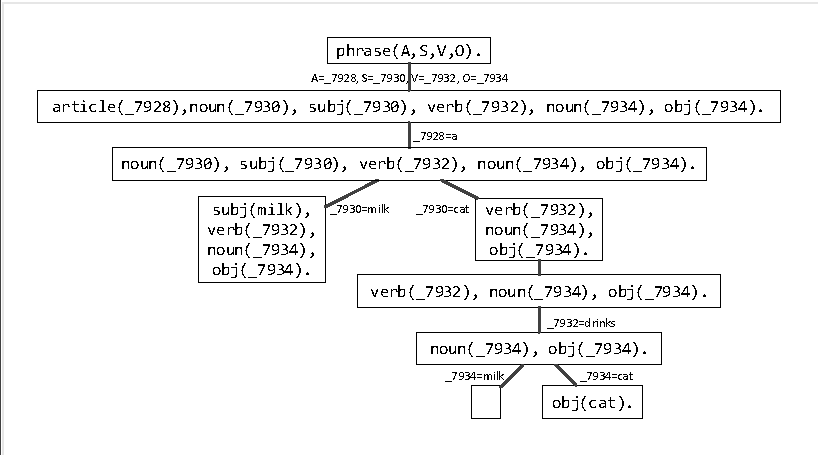
\includegraphics{prooftree}
	\end{figure}
\end{frame}


% Lesson 3. Recursion in Prolog
\lecture{Recursion}{recursion}

\section{Overview}

\begin{frame}
	\frametitle{\insertsection}
	Goals of the lesson
	\begin{itemize}
		\item Introduce recursive definitions in Prolog
		\item Discuss the mismatches between the declarative meaning of a Prolog program, and its procedural meaning
	\end{itemize}
\end{frame}


\section{Recursive definitions}

\begin{frame}
	\frametitle{\insertsection}
	Predicates can be defined recursively. It means that one or more rules in predicate's definition refers to itself.
	
	\only<1>{The most common example is a description of family relationships.}
	\only<2>{\textbf{Basis}}
	\only<3->{\textbf{Step}}
	
	\texttt{
		\begin{tabular}{l}
			{\color<2>[RGB]{255,0,0}{ancestor(Anc,Dec) :- child(Dec,Anc).}} \\
			{\color<3->[RGB]{255,0,0}{ancestor(Anc,Dec) :- child(Dec,Par), ancestor(Anc,Par).}} \\
			child(jane, peter). \\
			child(mary, kate). \\
			child(sam, mary). \\
			child(jason, jane). \\
			child(ann, jason).
		\end{tabular}
	}
\end{frame}


\begin{frame}
	\frametitle{\insertsection}
	
	Next, let us define natural numbers, having a definition of zero and a rule of succession. This representation is variously called successor arithmetic, successor notation and also \textbf{Peano arithmetic}.
	
	\texttt{
		\begin{tabular}{l}
			num(0). \\
			num(s(N)) :- num(N). \\ \\
			\uncover<2->{sum(0, N, N). \\
				sum(s(M), N, s(S)) :- sum(M, N, S).
			}
		\end{tabular}
	}

	\uncover<3->{Our numbers will be something like: \(0, s(0), s(s(0)), s(s(s(0))), \ldots\) Not very pleasant if you want to compute something, but sometimes used
	in automated provers.}
	
\end{frame}


\section{Tail recursion}

\begin{frame}
	\frametitle{\insertsection}
	
	Suppose we want to compute factorial (in normal numbers this time). We already know about recursion, and after a while will end up with a program similar to this one:
	
	\texttt{
		\begin{tabular}{l}
			f(0,1). \\
			f(N,F) :- N > 0, M is N - 1, f(M,Acc), F is Acc*N.
		\end{tabular}
	}

	Binary predicate \texttt{f/2} takes two arguments: natural number N and factorial of N. The table below shows possible queries.
	
	\texttt{\begin{table}\centering\begin{tabular}{l | l}
			f(4, F). & F = 24. \\
			\hline
			f(5, 120). & true. \\
			\hline
			f(X, 120). & ERROR \\
	\end{tabular}\end{table}}	
	
\end{frame}


\begin{frame}
	\frametitle{\insertsection}
	
	A recursive function is \textbf{tail recursive} when recursive call is the last thing executed by the function. It works in Prolog just well.
	Let us rewrite our factorial function, and make it tail recursive.
	
	\texttt{
		\begin{tabular}{l}
			f(N,N,F,F) :- !. \\
			f(N,M,Acc,F) :- M1 is M + 1, Acc1 is Acc * M1, f(N,M1,Acc1,F). \\
			factorial(N,F) :- f(N,1,1,F).
		\end{tabular}
	}

	As we can see predicate \texttt{f} takes 4 arguments now: natural number N, computation step M, result computed on step M, and total result F. Below are some examples.
	
	\texttt{\begin{table}\centering\begin{tabular}{l | l}
				factorial(4, F). & F = 24. \\
				\hline
				factorial(5, 120). & true. \\
				\hline
				factorial(X, 120). & X = 5. \\
	\end{tabular}\end{table}}	
	
\end{frame}


\section{Clause ordering, goal ordering, and termination}

\begin{frame}
	\frametitle{\insertsection}
	
	\only<1>{Recall our family program which as we know works just fine:}
	\only<2->{But what happens if we swap goals in the second rule?}
	\texttt{
		\begin{itemize}
			\item[] ancestor(Anc,Dec) :- child(Dec,Anc).
			\item<1>[] ancestor(Anc,Dec) :- child(Dec,Par), ancestor(Anc,Par).
			\item<2->[] \underline{ancestor(Anc,Dec) :- ancestor(Anc,Par), child(Dec,Par).}
			\item[] child(jane, peter).
			\item[] child(mary, kate).
			\item[] child(sam, mary).
			\item[] child(jason, jane).
			\item[] child(ann, jason).
		\end{itemize}
	}
	\uncover<2->{If we pose query \texttt{ancestor(jane, ann)} we will get a correct answer (\texttt{true}), and then an error message which means that Prolog is looping. }

\end{frame}

\begin{frame}
	\frametitle{\insertsection}
	\begin{figure}
		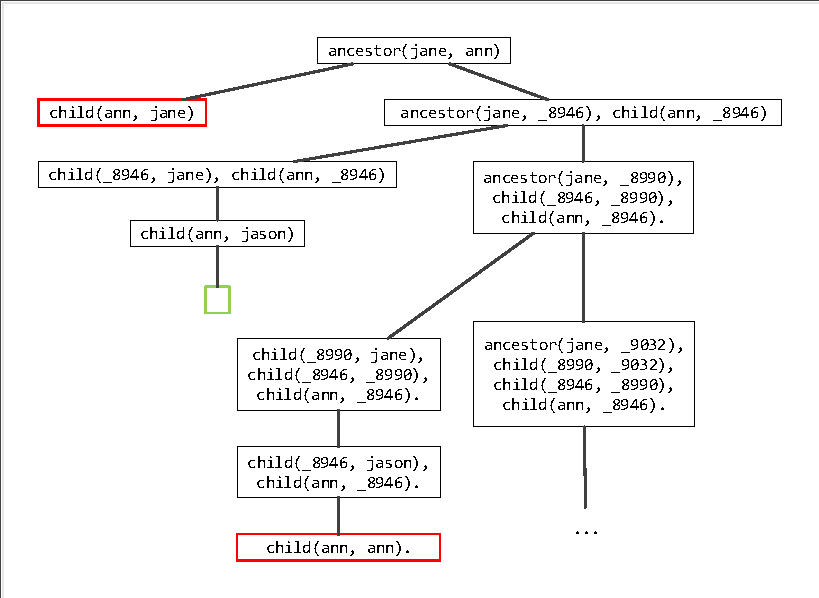
\includegraphics[scale=0.78]{badtree}
	\end{figure}
\end{frame}


% Lesson 5 Arithmetic in Prolog
\lecture{Arithmetic}{arithmetic}


\section{Overview}

\begin{frame}
	\frametitle{\insertsection}
	Goals of the lesson
	\begin{itemize}
		\item To introduce Prolog’s inbuilt abilities for performing arithmetic.
		\item To discuss how they can be applied to other data types' processing problems.
	\end{itemize}
\end{frame}


\section{Drawbacks of the successor arithmetic}

\begin{frame}
	\frametitle{\insertsection}
	
	Recall our Peano arithmetic implementation.
	
	\texttt{
		\begin{tabular}{l}
			num(0). \\
			num(s(N)) :- num(N).
		\end{tabular}
	}

	This is a pure predicate that terminates if any of the arguments is instantiated. We can read the clauses declaratively to reason about the cases that this relation describes. Other elementary relations between natural numbers can be defined analogously.
\end{frame}


\begin{frame}[shrink=4]
	\frametitle{\insertsection}
	
	Unfortunately, this representation of natural numbers suffers from several significant disadvantages:
	\begin{itemize}
		\item First, this is not really the way we want to write and read numbers. We would like to use a more familiar notation~--- such as 1, 2 and 3~--- to represent natural numbers.
		\item With some practice, we may get used to the successor notation. However, a more fundamental problem remains: This representation takes space that is directly proportional to the magnitude of the numbers we need to represent. Thus, the space requirement grows exponentially with the length of any number's decimal representation. Therefore, reasoning about larger numbers is infeasible with this representation.
		\item More complex relations such as multiplication and exponentiation are hard to define in such a way that they work in all directions and retain good termination properties.
		\item To extend this representation to integers, we also need a way to represent negative numbers.
	\end{itemize}
	
\end{frame}


\begin{frame}
	\frametitle{\insertsection}
	\justifying
	Therefore, successor notation~--- albeit useful to illustrate different ways in which we could represent our data~--- is not how we typically reason about numbers in Prolog.
\end{frame}


\begin{frame}
	\frametitle{\insertsection}
	\justifying
	Instead, we use built-in predicates to reason about numbers in Prolog. In the case of integers, these predicates are known as \textbf{CLP(FD)} constraints, and in more recent systems also as CLP(\(\mathds{Z} \)) constraints. CLP(FD) stands for \textbf{Constraint Logic Programming over Finite Domains} and reminds us of the fact that in reality, we can only represent a finite subset of integers on actual machines, while \(\mathds{Z} \) denotes the integers and indicates that these constraints are designed for reasoning about all integers.
	
	All widely used Prolog implementations provide CLP(FD) constraints. However, the exact details differ slightly between various systems. For example, in GNU Prolog, B-Prolog and other systems, CLP(FD) constraints are conveniently available right from the start. In contrast, you need to load a library to use them in SICStus Prolog and other systems.
	
	SWI Prolog provides a number of basic arithmetic tools for manipulating integers.
\end{frame}


\section{Arithmetic in Prolog}

\begin{frame}[shrink=3]
	\frametitle{\insertsection}
	
	SWI-Prolog defines the following numeric types:
	
	\begin{itemize}
		\item \textbf{Integer} If SWI-Prolog is built using the GNU multiple precision arithmetic library (GMP), integer arithmetic is unbounded, which means that the size of integers is limited by available memory only. Without GMP, SWI-Prolog integers are 64-bits, regardless of the native integer size of the platform. The inbuild predicate \texttt{integer/1} holds if
		an argument is an integer.
		\item \textbf{Rational number} Rational numbers (\(\mathds{Q} \)) are quotients of two integers (\(\frac{N}{M} \)). Rational arithmetic is only provided if GMP is used. Rational numbers satisfy the type tests \texttt{rational/1}, \texttt{number/1} and \texttt{atomic/1} and may satisfy the type test \texttt{integer/1}, i.e., integers are considered rational numbers. Rational numbers are always kept in canonical representation, which means \(M\) is positive and \(N\) and \(M\) have no common divisors.
		\item \textbf{Float} Floating point numbers are represented using the C type double. On most of today's platforms these are 64-bit IEEE floating point numbers. Satisfy the type tests \texttt{float/1}, \texttt{number/1} and \texttt{atomic/1}.
	\end{itemize}

\end{frame}


\begin{frame}
	\frametitle{\insertsection}
	
	\begin{table}
		\centering
		\begin{tabular}{ l | r }
			\rowcolor{Gray}
			\textbf{Arithmetic expression} & \textbf{Same in Prolog} \\
			\hline
			\rowcolor{LightGray}\( 10 + 5 = 15 \) & \texttt{15 is 10 + 5.}   \\
			\rowcolor{LightGray}\( 10\cdot 5 = 50 \)  & \texttt{50 is 10 * 5.}   \\
			\rowcolor{LightGray}\( 10 - 5 = 5 \)  & \texttt{5 is 10 - 5.}   \\
			\rowcolor{LightGray}\( 5 - 10 = -5 \)  & \texttt{-5 is 5 - 10.}   \\
			\rowcolor{LightGray}\( 10~/~5 = 2 \)  & \texttt{2 is 10 / 5.}   \\
			\rowcolor{LightGray}\( 10~/~4 = 2.5 \)  & \texttt{2.5 is 10 / 4.}   \\
			\rowcolor{LightGray}\( 10~/~4 = 4\cdot 2 + 2 \)  & \texttt{2 is mod(10,4).}  \\
		\end{tabular}
	\end{table}
	
\end{frame}


\begin{frame}
	\frametitle{\insertsection}
	
	\begin{table}
		\centering
		\begin{tabular}{ l | r }
			\rowcolor{Gray}
			\textbf{Arithmetic expression}   & \textbf{Same in Prolog} \\
			\hline
			\rowcolor{LightGray}\( x < y \) & \texttt{X < Y.}  \\
			\rowcolor{LightGray}\( x\leqslant y \)  & \texttt{X =< Y.}   \\
			\rowcolor{LightGray}\( x = y \)  & \texttt{X =:= Y.}  \\
			\rowcolor{LightGray}\( x\neq y \)  & \texttt{X =\textbackslash = Y.}  \\
			\rowcolor{LightGray}\( x\geqslant y \)  & \texttt{X >= Y.}  \\
			\rowcolor{LightGray}\( x > y \)  & \texttt{X > Y.} \\
		\end{tabular}
	\end{table}
	
\end{frame}


\begin{frame}
	\frametitle{\insertsection}
	
	SWI-Prolog provides many extensions to the set of floating point functions defined by the ISO standard.
	
	\begin{example}
		\texttt{sin, cos, tan, log, log10, exp, **, sqrt, ceil, floor, round, abs, max, min, >>, <<}
	\end{example}
\end{frame}


\begin{frame}
	\frametitle{\insertsection}
	
	Normally all Prolog does is just unification of variables to structures. Arithmetic is something extra that has been bolted on to the basic Prolog engine because it is useful.
	
	Arithmetic functions are terms which are evaluated by the arithmetic predicates. Apart from the fact that the functors go between their	arguments instead of in front of them these are ordinary Prolog terms, and unless we	do something special, Prolog will not actually do any arithmetic.
	
	To force Prolog to actually evaluate arithmetic	expressions we have to use inbuild binary predicate \texttt{is/2}.
	
\end{frame}


\begin{frame}
	\frametitle{\insertsection}
	
	Since arithmetic functions is an extra stuff in Prolog then it is not surprising that there are some restrictions on this extra ability.
	
	\begin{itemize}
		\item The arithmetic expressions to be evaluated must be on the right hand side of \texttt{is}.
		\item Moreover, every variable on the right hand side must already have been instantiated to a number. If the variable is uninstantiated, or if it is instantiated to something
		other than a number, we will get some sort of \texttt{instantiation\_error} message.
	\end{itemize}

\end{frame}


\begin{frame}
	\frametitle{\insertsection}
	
	Here’s an example.
	
	\texttt{double(N, D) :- D is N * 2.}
	
	This predicate simply doubles its first argument and returns the answer in its second argument.
	
	\begin{itemize}
		\item \texttt{double(5, A)} returns \texttt{A = 10.}
		\item But posing the query \texttt{double(Half, 10)} does not return anything. Instead we get the \texttt{instantiation\_error} message. When we pose the query, we are asking Prolog
		to evaluate expression \texttt{10 is Half * 2}, which is impossible due to uninstantiation of \texttt{Half}.
	\end{itemize}
	
	\begin{example}
		\texttt{15 is 10 + 5.} \(\Leftrightarrow \) \texttt{is(15,+(10,5)).} \\
		\texttt{X is (2*5 + 10) / 4.} \(\Leftrightarrow \) \texttt{is(X,/(+(*(2,5),10),4)).}
	\end{example}
\end{frame}


% Lesson 6. Lists
\lecture{Lists}{lists}


\section{Overview}

\begin{frame}
	\frametitle{\insertsection}
	Goals of the lesson
	\begin{itemize}
		\item To introduce lists, an important recursive data structure widely used in computational linguistics.
		\item To define predicates Prolog provides to work with lists.
		\item To introduce the idea of recursing down lists.
	\end{itemize}
\end{frame}


\section{Functional notation}

\begin{frame}
	\frametitle{\insertsection}
	
	Lists are Prolog terms for which there are dedicated syntactic provisions.
	
	Lists are defined inductively:
	
	\begin{itemize}
		\item The atom \texttt{[]} (nil) is a list. It denotes an empty list.
		\item The compound term \texttt{.(H, T)} is a list iff \texttt{T} is a list. \texttt{H} is a first element or \textbf{head} of the list, and \texttt{T} is a \textbf{tail} of the list.
	\end{itemize}

	As if to make canonical definition of lists more painful in SWI Prolog predicate \texttt{'[|]'} is used instead of \texttt{'.'}.
\end{frame}

\begin{frame}
	\frametitle{\insertsection}
	
	\begin{table}
		\begin{center}
			\begin{tabular}{m{5cm} c}
				\only<1>{
					\texttt{[]}
					&
					An empty list
				}
				\only<2>{
					\texttt{'[|]'(a,[])}
					& 
					\begin{tabular}{c}
						\raisebox{-\totalheight}{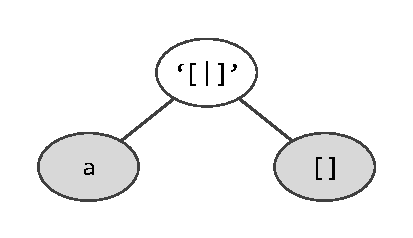
\includegraphics[scale=1.3]{list1}}
					\end{tabular}
				}
				\only<3>{
					\texttt{'[|]'(a, '[|]'(b, []))}
					&
					\begin{tabular}{c}
						\raisebox{-\totalheight}{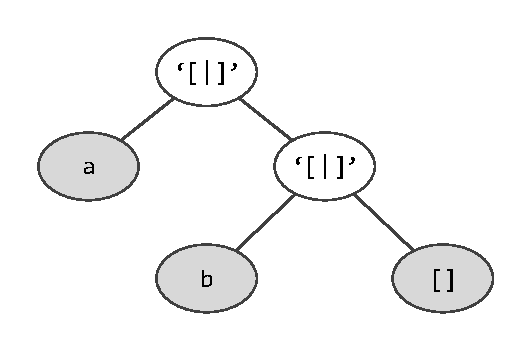
\includegraphics{list2}}
					\end{tabular}
				}
			\end{tabular}
		\end{center}
	\end{table}
\end{frame}


\section{List notation}

\begin{frame}
	\frametitle{\insertsection}
	
	\begin{itemize}
		\item List is a finite sequence of elements.
		\item Lists in Prolog are specified by enclosing the elements in square brackets [...].
		\item The elements are separated by commas: \texttt{[one, two, three, 1, 2]}. The length of a list is a number of its elements. Any term could be an element of a list.
		\item Any non-empty list can be thought of as consisting of the head and the tail. The head is simply the first item in the list; the tail is everything else. SWI Prolog has a special inbuilt operator | which can be used to decompose a list into its head and tail.
		\item The empty list contains no internal structure.
	\end{itemize}

\end{frame}


\begin{frame}
	\frametitle{\insertsection}
	
	\begin{table}
		\begin{center}
			\begin{tabular}{m{3cm} c}
				\only<1>{
					\texttt{[]}
					&
					An empty list
				}
				\only<2>{
					\texttt{[a]}
					& 
					\begin{tabular}{c}
						\raisebox{-\totalheight}{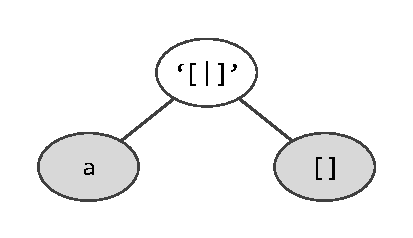
\includegraphics[scale=1.3]{list1}}
					\end{tabular}
				}
				\only<3>{
					\texttt{[a, b]}
					&
					\begin{tabular}{c}
						\raisebox{-\totalheight}{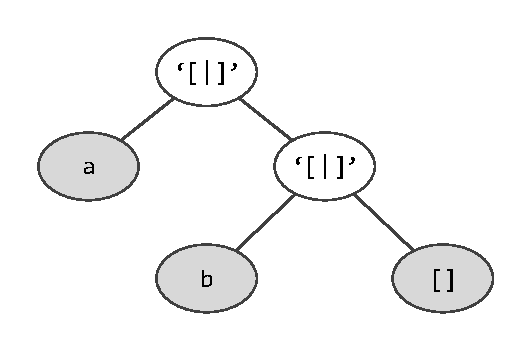
\includegraphics{list2}}
					\end{tabular}
				}
				\only<4>{
					\texttt{[a, b, c]}
					&
					\begin{tabular}{c}
						\raisebox{-\totalheight}{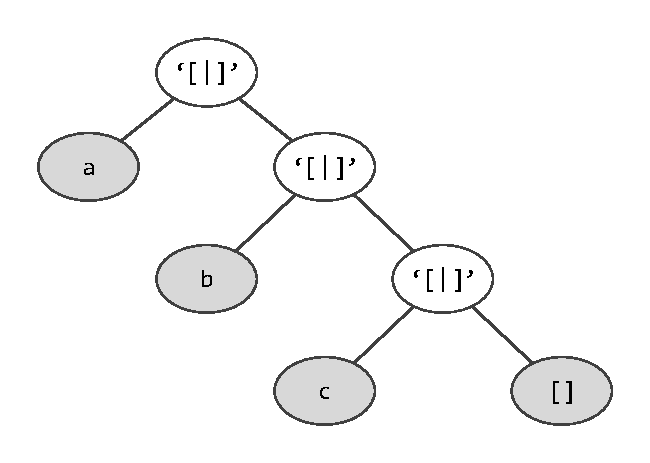
\includegraphics[scale=0.88]{list3}}
					\end{tabular}
				}
			\end{tabular}
		\end{center}
	\end{table}
\end{frame}


\begin{frame}
	\frametitle{\insertsection}
	
	\texttt{\begin{itemize}
			\item[] []
			\item[] [first, second, third, fourth, fifth]
			\item[] [1, 2, 3, 4, 5, 6, 7, 8, 9, 0]
			\item[] [first, 2, color(cornie, black), F, fifth, F]
			\item[] [first, second, [third, fourth], [fifth, color(cornie, black)]]
			\item[] [[], [], car(volkswagen), F, 1, 2, [1, F, car(bmw), [1, 2, 4]], X]
	\end{itemize}}
\end{frame}


\section{Elements and operations}

\begin{frame}
	\frametitle{\insertsection}
	
	\texttt{\begin{itemize}
			\item[] [abyssian, bobtail, [bengal, birman]]
	\end{itemize}}
	
	\texttt{\begin{itemize}
			\item<2-> {[H|T]} = [abyssian, bobtail, [bengal, birman]].
			\item<3-> {[F,S|T]} = [abyssian, bobtail, [bengal, birman]].
			\item<4-> {[\_,S|T]} = [abyssian, bobtail, [bengal, birman]].
			\item<5-> {[First,\_,\_,Fourth|\_]} = [abyssian, bobtail, [bengal, birman]].
			\item<6-> {[\_,\_,[\_|T]|\_]} = [abyssian, bobtail, [bengal, birman]].
	\end{itemize}}
	
\end{frame}


\begin{frame}
	\frametitle{\insertsection}
	
	The inbuilt predicate \texttt{member/2 = member(?Elem, ?List)} is True if \texttt{Elem} is a member of \texttt{List}, and False otherwise.
	
	\texttt{\begin{table}\centering\begin{tabular}{l | l}
		member(a, []). & false. \\
		\hline
		member(a, [b, a, 1, [], f(a, b, c)]) & true
	\end{tabular}\end{table}}

	\texttt{\begin{itemize}
			\item<2->[] member(X, [X|T]).
			\item<3->[] member(X, [H|T]) :- member(X,T).
	\end{itemize}}
	
	\uncover<4->{\texttt{\begin{itemize}
				\item[] member(X, [X|\_]).
				\item[] member(X, [\_|T]) :- member(X,T).
	\end{itemize}}}
\end{frame}


\begin{frame}
	\frametitle{\insertsection}
	
	Other operations on lists:
	
	\begin{enumerate}
		\item Length of a list.
		\item Concatenation.
		\item Prefix, suffix and a sublist of a list.
		\item Get last element.
		\item List reversal.
		\item Sorting.
	\end{enumerate}
\end{frame}


% Lesson 7. Dynamic database
\lecture{Database}{db}

\section{Overview}

\begin{frame}
	\frametitle{\insertsection}
	Goals of the lesson
	\begin{itemize}
		\item Define a predicate which causes one or more clauses to be added to or deleted from the Prolog database.
		\item Define predicates to create and manipulate a database of related facts within the Prolog database.
		\item To discuss inbuilt predicates that let us collect all solutions to a problem into a single list.
	\end{itemize}
\end{frame}

\section{Database}

\begin{frame}
	\frametitle{\insertsection}
	
	The normal way of placing clauses in the Prolog database is to consult or reconsult one or more files.
	
	A consult directive causes all the clauses in the file to be loaded into the knowledge base to add to those already there. A reconsult directive behaves in a similar way to consult, with one crucial	difference. If any clause in the reconsulted file is for the same predicate as a clause	already in the database (i.e. their heads have the same functor and arity), all clauses
	for that predicate in the database are first deleted.
	
	Clauses placed into the knowledge base normally stay there until added to or deleted by a subsequent consult or reconsult directive, or until the user exits from the Prolog system when all clauses are automatically deleted. For most purposes this is entirely sufficient.
\end{frame}


\begin{frame}
	\frametitle{\insertsection}
	
	However Prolog also has built-in predicates for adding clauses to and deleting clauses from the database which can be useful for more advanced programming in the language. Like many other 'advanced' features, they need to be used with care.
	
	As usual, these built-in predicates can be used either in the body of a rule or in a directive entered at the system prompt. As the user's program and the Prolog database are equivalent, using them in the body of a clause is equivalent to modifying the user's program while it is being used.
\end{frame}


\begin{frame}
	\frametitle{\insertsection}
	
	SWI-Prolog offers predicates to manage knowledge base during the execution of Prolog programs.
	\texttt{\begin{itemize}
			\item assert/1
			\item asserta/1
			\item assertz/1
			\item retract/1
			\item retractall/1
			\item abolish/1
	\end{itemize}}

	There are others, of cause. You can become acquainted with them here: \href{https://www.swi-prolog.org/pldoc/man?section=db}{https://www.swi-prolog.org/pldoc/man?section=db}
\end{frame}


\begin{frame}
	\frametitle{\insertsection}
	
	If any predicate is to be modified using \texttt{assertz}, \texttt{retract} etc., it should be specified as \textbf{dynamic} by a directive in the user's program. 
	As an example, for predicate \texttt{f} with arity 2, the line
	
	\texttt{:- dynamic(f/3).}
	
	should be added at or near the start of the program and certainly before the first clause that mentions the \texttt{f} predicate.
	
	If the dynamic directive is left out, attempts to modify the database are likely to produce error messages such as \textit{''Predicate Protected``} or even \textit{''Predicate Not Defined``}.
\end{frame}


\begin{frame}
	\frametitle{\insertsection}
	
	Suppose we start with an empty database. So if we give the command:
	
	\texttt{?- listing.}
	
	we simply get a \texttt{true.}; the listing is empty, except for the garbage it always prints for no sane reason. Suppose we now give this command:
	
	\texttt{?- assert(f(x,y)).}
	
	It succeeds (\texttt{assert} commands \textbf{always succeed}). But what is important is the side-effect it has on the database. If we now give the command:
	
	\texttt{?- listing.}

	we get the listing:
	
	\texttt{:- dynamic f/2.\\f(x,y).}
\end{frame}


\begin{frame}
	\frametitle{\insertsection}
	
	We can do the same thing with rules as well. Rules must be enclosed in an additional pair of parentheses.
	
	\texttt{?- assert((f(X,y) :- X > 5)).}
	
	As you can see, the clause used for the argument should be written without a terminating full stop.
	
	Now we may pose query like:
	
	\texttt{?- f(10, y).}
	
	and get an answer \texttt{true.}
	
	\textbf{Note that clauses will occur in the knowledge base as many times as they were asserted.}
\end{frame}


\begin{frame}
	\frametitle{\insertsection}
	
	Two main predicates available for deleting clauses from the database are:
	
	\texttt{\begin{itemize}
			\item retract(?Clause)
			\item retractall(?Clause)
	\end{itemize}}
	
\end{frame}


\begin{frame}[shrink=7]
	\frametitle{\insertsection}
	
	The predicate \texttt{retract/1} takes a single argument, which must be a clause, i.e. a fact or a rule. It causes the first clause in the database that matches (i.e. unifies with) \texttt{Clause} to be deleted. If the following clauses are in the database
	
	\texttt{dog(jim).\\dog(fido).\\dog(X).}
	
	the query
	
	\texttt{?- retract(dog(fido)).}
	
	will delete the second clause and the further query
	
	\texttt{?-retract(dog(X)).}
	
	will delete the \texttt{dog(jim)} clause, which is the first one of the remaining two clauses to unify with the query. This will leave the \texttt{dog(X)} clause in the database. Although unusual, this is a valid Prolog fact which signifies 'everything is a dog'.
	
\end{frame}


\begin{frame}[shrink=7]
	\frametitle{\insertsection}
	
	The predicate \texttt{retractall/1} takes a single argument which must be the head of a clause. It causes every clause in the database whose head matches \texttt{Clause} to be
	deleted. The \texttt{retractall} goal always succeeds even if no clauses are deleted. Some examples are:
	
	\texttt{?- retractall(f(\_,\_)).}
	
	which deletes all the clauses for the \texttt{f/2} predicate, and
	
	\texttt{?- retractall(parent(john,Y)).}
	
	which deletes all clauses for the \texttt{parent/2} predicate which have the atom \texttt{john} as their first argument. Note that the directive
	
	\texttt{?- retractall(f).}
	
	only removes the clauses for predicate \texttt{f/0}. To delete all the clauses for predicate \texttt{f/2} it is necessary to use
	
	\texttt{?- retractall(f(\_,\_)).}
\end{frame}


\section{Database: Examples}

\begin{frame}
	\frametitle{\insertsection}
	
	\only<1>{Let us take an empty database and add some facts and one rule to it:
		
		\texttt{\begin{itemize}
				\item[] ?- assertz(f(x,y)).
				\item[] ?- assertz(f(x,y)).
				\item[] ?- assertz(f(a,b)).
				\item[] ?- assertz((f(X,y) :- g(X,a,b)).
	\end{itemize}}}
	
	\only<2>{Now if we pose a query \texttt{?- listing(f/2).} we will get
		
		\texttt{\begin{itemize}
				\item[] :- dynamic f/2.
				\item[] f(x,y).
				\item[] f(x,y).
				\item[] f(a,b).
				\item[] f(X,y) :- g(X,a,b).
	\end{itemize}}}
	
	\only<3>{Let us now delete one occurrence of the fact \texttt{f(x,y)}.
		
		\texttt{\begin{itemize}
				\item[] retract(f(x,y)).
				\item[]
				\item[] f(x,y).
				\item[] f(a,b).
				\item[] f(X,y) :- g(X,a,b).
	\end{itemize}}}
	
	
	\only<4>{From what is left in database we delete all facts and rules such that their head is matched with \texttt{f(X,y)}.
		
		\texttt{\begin{itemize}
				\item[] retractall(f(X,y)).
				\item[]
				\item[] f(a,b).
	\end{itemize}}}

\end{frame}


\begin{frame}
	\frametitle{\insertsection}
	
	Consider another example:
	
	\texttt{\begin{tabular}{l l}
			multab(Scale) :- & member(X,Scale),\\
			~ & member(Y,Scale),\\
			~ & P is X * Y,\\
			~ & assertz(p(X,Y,P)),\\
			~ & fail.
	\end{tabular}}
\end{frame}


\section{Database: Conclusions}

\begin{frame}
	\frametitle{\insertsection}
	
	\begin{itemize}
		\item You have to define predicate as dynamic in order to use it with \texttt{asserta, assertz, retract} and \texttt{retractall}.
		\item If predicate \texttt{p} is not yet defined in the database it will be defined as dynamic when first used in \texttt{assert} operation.
		\item Predicate \texttt{abolish/1} removes all clauses of a predicate from the database. All predicate attributes (dynamic, multifile, index, etc.) are reset to their defaults. According to the ISO standard, \texttt{abolish/1} can only be applied to dynamic procedures. This is odd, as for dealing with dynamic procedures there is already \texttt{retract/1} and \texttt{retractall/1}. The \texttt{abolish/1} predicate was introduced in DEC-10 Prolog precisely for dealing with static procedures. In SWI-Prolog, \texttt{abolish/1} works on static procedures, unless the Prolog flag iso is set to true. \textbf{It is advised to use \texttt{retractall/1} for erasing all clauses of a dynamic predicate.}
	\end{itemize}
\end{frame}


\section{Aggregation}

\begin{frame}
	\frametitle{\insertsection}
	
	There may be more than one solution to a query. Prolog interpreter, however, returns solutions one by one. Sometimes we would like to have all the solutions to a query at once, and we would like them handed to us on a pretty usable form. Prolog has 3 built-in predicates that do precisely this:
	\texttt{\begin{itemize}
			\item findall/3
			\item bagof/3
			\item setof/3
	\end{itemize}}
	
	Basically these predicates collect all the solutions to a query and put them in a list, but	there are important differences between them.
	
\end{frame}


\begin{frame}
	\frametitle{\insertsection}
	
	The query
	
	\texttt{?- findall(Buffer, Goal, Response).}
	
	produces a list \texttt{Response} of all the objects of a form of \texttt{Buffer} that satisfy the goal \texttt{Goal}. Often \texttt{Buffer} is simply a variable, in which case the query can be read as: \textbf{Give me a list containing all the instantiations of Object which satisfy Goal.}
	
	If there are no solutions satisfying the \texttt{Goal} the \texttt{findall} predicate returns an empty list as response.
	
\end{frame}


\begin{frame}
	\frametitle{\insertsection}
	
	Suppose we want to get a subset of our little multiplication table we made:
	
	\texttt{\begin{tabular}{m{13cm}}
			?- findall([X,Y], p(9, X, Y), Response).\\
			Response = [[1, 9], [2, 18], [3, 27], [4, 36], [5, 45], [6, 54], [7, 63], [8|...], [...|...]].\\\\
			?- findall(9 * X = Y, p(9, X, Y), Response).\\
			Response = [9*1=9, 9*2=18, 9*3=27, 9*4=36, 9*5=45, 9*6=54, 9*7=63, ... * ... = 72, ... = ...].\\
	\end{tabular}}
	
\end{frame}


\begin{frame}
	\frametitle{\insertsection}
	
	The \texttt{bagof/3} predicate is more finegrained than \texttt{findall}, it gives us the opportunity to extract the information we want in a more structured way. Moreover, \texttt{bagof} can also do the same job as \texttt{findall}, with the help of a special piece of syntax.
	\only<1>{\texttt{\begin{table}\centering\begin{tabular}{|l | l|}
			\hline
			\multirow{5}{4cm}{?- bagof(pair(X,Y), p(X,Y,Z), R).} & Z = 1, R = [pair(1, 1)] ;\\
			& Z = 2, R = [pair(1, 2), pair(2, 1)] ;\\
			& Z = 3, R = [pair(1, 3), pair(3, 1)] ;\\
			& Z = 4, R = [pair(1, 4), pair(2, 2), pair(4, 1)] ;\\
			& Z = 5, R = [pair(1, 5), pair(5, 1)] ;\\
			\hline
	\end{tabular}\end{table}}}
	\only<2->{
		\texttt{\begin{table}\centering\begin{tabular}{|l | l|}
				\hline
				\multirow{4}{*}{?- bagof(X, p(X, Y, Z), R).} & Y = Z, Z = 1, R = [1] ;\\
				& Y = 1, Z = 2, R = [2] ;\\
				& Y = 1, Z = 3, R = [3] ;\\
				& Y = 1, Z = 4, R = [4] ;\\
				\hline
				\multirow{6}{*}{?- bagof(X, Y\textasciicircum p(X, Y, Z), R).} & Z = 1, R = [1] ;\\
				& Z = 2, R = [1, 2] ;\\
				& Z = 3, R = [1, 3] ;\\
				& Z = 4, R = [1, 2, 4] ;\\
				& Z = 5, R = [1, 5] ;\\
				& Z = 6, R = [1, 2, 3, 6] ;\\
				\hline
		\end{tabular}\end{table}}
	}
	
\end{frame}


\begin{frame}
	\frametitle{\insertsection}
	
	The \texttt{setof/3} predicate is basically the same as \texttt{bagof}, but with one useful difference: the lists it contains are ordered and contain no redundancies. \textbf{That is, each item appears in the list only once.}
	
	\texttt{\begin{tabular}{|l | m{7cm}|}
			\hline
			?- findall(Y, p(X, Y, Z), R). & R =  [1, 2, 3, 4, 5, 6, 7, 8, 9, 1, 2, 3, 4, 5, 6, 7, 8, 9, 1, 2, 3, 4, 5, 6, 7, 8, 9, 1, 2, 3, 4, 5, 6, 7, 8, 9, 1, 2, 3, 4, 5, 6, 7, 8, 9, 1, 2, 3, 4, 5, 6, 7, 8, 9, 1, 2, 3, 4, 5, 6, 7, 8, 9, 1, 2, 3, 4, 5, 6, 7, 8, 9, 1, 2, 3, 4, 5, 6, 7, 8, 9].\\
			\hline
			?- setof(Y, X\textasciicircum Z\textasciicircum p(X, Y, Z), R). & R = [1, 2, 3, 4, 5, 6, 7, 8, 9].\\
			\hline
	\end{tabular}}
	
\end{frame}


\section{Conclusions}

\begin{frame}
	\frametitle{\insertsection}
	
	\begin{itemize}
		\item Dynamic database allows to cache solutions and manipulate facts and rules in runtime.
		\item Typically it is a bad idea to overuse the database manipulation predicates as it hampers considerably program tracing and debug. Nevertheless, there are scenarios where storing data outside the Prolog stacks is a good option.
		\item Typically, first consider representing data processed by your program as terms passed around as predicate arguments. If you need to reason over multiple solutions to a goal, consider \texttt{findall/3}, and related predicates.
	\end{itemize}
	
\end{frame}



% Lesson 8. Files
\lecture{Files}{files}

\section{Overview}

\begin{frame}
	\frametitle{\insertsection}
	Goals of the lesson
	\begin{itemize}
		\item How predicate definitions can be spread across different files
		\item How to write results to files and how to read input from files
	\end{itemize}
\end{frame}


\section{Splitting programs over modules}

\begin{frame}
	\frametitle{\insertsection}
	
	
	By now, you have seen and you had to write lots of programs that use miscellaneous predicates you described. What you probably did each time you needed one of them was
	to go back to the definition and copy it over into the file where you wanted to use it. And maybe, you started thinking that it would be a lot nicer if you could define them somewhere once and for all and then just access that definition whenever you needed it.
	
	That sounds like a pretty sensible thing to ask for and, of course, Prolog offers ways of doing it.
		
\end{frame}


\begin{frame}
	\frametitle{\insertsection}
	
	If you want Prolog to consult an extra code you have to place a list of files at the beginning of your program like this:
	
	\only<1>{\texttt{
		\begin{tabular}{l}
			:- [sourceCode1, sourceCode2, \ldots].
		\end{tabular}}

		Doing so you are telling Prolog to consult the files in the square brackets before reading in the rest of the file. 
		
		On encountering something of such the form, Prolog just goes
		ahead and consults the files without checking whether the file really needs to be consulted. If the predicate definitions provided by one of the files are already
		available, because it already was consulted once, Prolog still consults it again, overwriting the definitions in the database.
	}
	\only<2->{
		\texttt{
			\begin{tabular}{l}
				:- ensure\_loaded([sourceCode1, sourceCode2, \ldots]).
			\end{tabular}
		}
	
	
		The inbuilt predicate \texttt{ensure\_loaded/1} behaves more clever in this case and it is what you should usually use to load predicate definitions given in some other file into your program.
		
		On encountering the following directive \texttt{:- ensure\_loaded([sourceCode1, sourceCode2]).} Prolog checks whether the files \texttt{sourceCode1.pl} and \texttt{sourceCode2.pl} have already been loaded. If not, Prolog loads them. If they already are loaded in, Prolog checks whether something has changed since last loading them and if that is the case, Prolog loads them, if not, it doesn’t do anything and goes on processing the program.
	}
	
	
\end{frame}


\begin{frame}
	\frametitle{\insertsection}
	
	Imagine that you are writing a program that needs two predicates \texttt{f/1} and \texttt{g/2}. You described \texttt{f/1} and \texttt{g/2} in the files
	\texttt{source1.pl} and \texttt{source2.pl} respectively. Now you can load this two files as we did before by putting
	
	\texttt{
		\begin{tabular}{l}
			:- ensure\_loaded([source1, source2]).
		\end{tabular}
	}

	at the top of your next program. Now, imagine that each of them depends on predicate \texttt{some\_helper/2}, which is defined both in \texttt{source1.pl} and \texttt{source2.pl}.
	
	Unfortunately, there seem to be problems this time. You get a message that looks something like:
	
	\texttt{
		\begin{tabular}{l}
			\alert{The procedure some\_helper/2 is being redefined} \\
			\alert{Do you really want to redefine it? (y, n, p, or ?)}
		\end{tabular}
	}
		
\end{frame}


\begin{frame}
	\frametitle{\insertsection}
	
	So what has happened? 
	
	Both files are defining the predicate \texttt{some\_helper/2}. And what’s worse, you can’t be sure that the predicate is defined in the same way in both files. So, you can’t just say <<yes, override>>, since \texttt{f/1} depends on the definition of \texttt{some\_helper/2} given in file \texttt{source1.pl} and \texttt{g/2} depends on the definition given in file \texttt{source2.pl}.
	
	Furthermore, note that you are not really interested in the definition of \texttt{some\_helper/2} at all. You don’t want to use it. The predicates that you are interested in, that you want to use are \texttt{f/1} and \texttt{g/2}. They need definitions of \texttt{some\_helper/2}, but the rest of your program doesn’t.
	
\end{frame}


\begin{frame}
	\frametitle{\insertsection}
	
	Instead of consulting the whole file we can turn it into a \textit{module}.
	
	Modules allow you to encapsulate predicate definitions. You are allowed to decide what is public and what is private in the module. 
	
	Public predicates are callable from outside of the module, while private are not. You are not allowed to call private predicates from somewhere except of the module itself, but there will be no conflicts if multiple modules internally define the same predicate.
	
	In our example \texttt{some\_helper/2} is a good candidate for becoming a private predicate.
	
\end{frame}


\begin{frame}
	\frametitle{insertsection}
	
	You can turn a source file into a module by putting a declaration of the following form at the top of that file:
	
	\texttt{\begin{tabular}{l}
			:- module(Name, ListOfPublicPredicates).
	\end{tabular}}
	
	This declaration specifies the name of the module and the list of predicates that should be declared public. That is, the list of predicates that you want to export.
	
	By putting
	
	\texttt{\begin{tabular}{l}
			:- module(source1, [f/1]). or \\
			:- module(source2, [g/2]).
	\end{tabular}}
	
	at the top of the corresponding file we define our modules. Predicate \texttt{some\_helper/2} is now hidden, so there is no clash when loading both modules at the same time.	 
	
\end{frame}


\begin{frame}
	\frametitle{\insertsection}
	
	Modules are loaded with the built-in predicate \texttt{use\_module/1}. Putting
	
	\texttt{\begin{tabular}{l}
			:- use\_module(source1).\\
			:- use\_module(source2).
	\end{tabular}}
	
	at the top of a source file will import all public predicates from both modules.
	
	Moreover, if you don't need all public predicates of a module, you can use the binary predicate \texttt{use\_module/2}, which takes the list of predicates you want to import from a module.
	
	\texttt{\begin{tabular}{l}
			:- use\_module(source1, [f/1]).\\
			:- use\_module(source2, [g/2]).
	\end{tabular}}
	
\end{frame}


\begin{frame}
	\frametitle{\insertsection}
	
	Many of the very common predicates are actually predefined in most Prolog implementations in one way or another. 
	
	If you have been using SWI Prolog, for example, you will probably have noticed that things like append and member are built in. That’s a specialty of SWI, however. Other Prolog implementations, like Sicstus for example, don’t have them built in. But they usually come with a set of libraries, i.e. modules defining common predicates. 
	
	These libraries can be loaded using the normal commands for importing modules. When specifying the name of the library that you want to use, you have to tell Prolog that this module is a library, so that Prolog knows where to look for it (namely, not in the directory where your other code is, but at the place where Prolog keeps its libraries).
	
\end{frame}


\begin{frame}
	\frametitle{\insertsection}
	
	Putting
	
	\texttt{\begin{tabular}{l}
			:- use\_module(library(libname)).
	\end{tabular}}
	
	at the top of your file tells Prolog to load a library having a name \texttt{libname}.
	
	Note, however, that the way libraries are organized and the inventory of predicates provided by libraries are by no means standardized across different Prolog implementations. In fact, the library systems may differ quite a bit.
	
	So, if you want your program to run with different Prolog implementations, it might be easier and faster to define your own library modules (using the techniques that we saw in the last section) than to try to work around all the incompatibilities between the library systems of different Prolog implementations.	
	
\end{frame}


\section{Writing to and reading from files}


\begin{frame}
	\frametitle{\insertsection}
	
	Now, we know how to load program code from files, and we want to look at reading an input data from files and outputting results to files.
	
	Before we can perform any actions on a file, we have to open it and associate a stream with it. Streams have names, that we can use to specify which stream to write or read from.
	Prolog assigns these names to streams, and all you need to do is bind them to a variables and then pass these variables around.
	
	The built-in predicate \texttt{open/3} opens a files and assign a stream with it.
	
	\texttt{\begin{tabular}{l}
			open(+FileName, +Mode, -Stream)
	\end{tabular}}

	The first argument is the name of the file, and in the last argument, Prolog returns the name this it assigns to the stream. Mode is one of \textit{read}, \textit{write} or \textit{append}.
	
\end{frame}


\begin{frame}
	\frametitle{\insertsection}
	
	When you are finished working with file, you should close it again. This is done by the built-in predicate \texttt{close/1}. It takes the name of the stream associated with file.
	
	Working-with-file session usually has the following structure:
	
	\texttt{\begin{tabular}{l}
			open(myfile, write, Stream).\\
			\ldots \\
			write something to the file \\
			\ldots \\
			close(Stream).
	\end{tabular}}
	
\end{frame}


\begin{frame}
	\frametitle{\insertsection}
	
	The predicates for writing to and reading from a stream are almost the same as the ones we already used. We have \texttt{write}, \texttt{writeln}, \texttt{read}, \texttt{nl}, etc.
	The only thing that is different is that we always give the stream that we want to write to or read from as the first argument.
	
	\texttt{\begin{tabular}{l l}
			readFile :- & open('in.txt',read,In),\\
			~ & \textbackslash+ at\_end\_of\_stream(In),\\
			~ & read(In,R),\\
			~ & writeln(In, R),\\
			~ & close(In).\\
			writeFile :- & open('../out.txt',write,Out),\\
			~ & write(Out, 'Some string.'),\\
			~ & write(Out, 'Skin(Smith,Black).'),\\
			~ & close(Out).
	\end{tabular}}
	
\end{frame}


% Lesson 9. Definite Clause Grammars
\lecture{DCG}{dcg}


\section{Overview}

\begin{frame}
	\frametitle{\insertsection}
	Goals of the lesson
	\begin{itemize}
		\item To introduce context free grammars (CFGs) and some related concepts.
		\item To introduce definite clause grammars (DCGs), an inbuilt Prolog mechanism	for working with context free grammars.
	\end{itemize}
\end{frame}


\section{Context free grammars}

\begin{frame}
	\frametitle{\insertsection}
	
	Prolog's inventor, Alain Colmerauer, was a computational linguist, and computational linguistics remains a classic application for
	the language. SWI Prolog offers a number of tools which make life easier for computational linguists, and today we are going to start
	learning about one of the most useful of these: Definite Clauses Grammars, or DCGs as they are usually called.
	
	In formal language theory, a \textbf{grammar} describes how to form strings from a language's alphabet that are valid according to the language's syntax. 
	A grammar does not describe the meaning of the strings or what can be done with them in whatever context—only their form. 
	
	A \textbf{formal grammar} is defined as a set of production rules for strings in a formal language.
	
\end{frame}


\begin{frame}
	\frametitle{\insertsection}
	
	\begin{table}
		\centering
		\begin{tabular}{ l }
			\rowcolor{LightGray} S \(\rightarrow \) nounPhrase verbPhrase \\
			\rowcolor{LightGray} nounPhrase \(\rightarrow \) article noun \\
			\rowcolor{LightGray} verbPhrase \(\rightarrow \) verbExpr nounPhrase \\
			\rowcolor{LightGray} verbExpr \(\rightarrow \) modalVerb verb prep \\
			\rowcolor{LightGray} article \(\rightarrow \) a \\
			\rowcolor{LightGray} article \(\rightarrow \) the \\
			\rowcolor{LightGray} noun \(\rightarrow \) cat \\
			\rowcolor{LightGray} noun \(\rightarrow \) king \\
			\rowcolor{LightGray} modalVerb \(\rightarrow \) may \\
			\rowcolor{LightGray} verb \(\rightarrow \) look \\
			\rowcolor{LightGray} prep \(\rightarrow \) at
		\end{tabular}
	\end{table}
\end{frame}


\begin{frame}
	\frametitle{\insertsection}
	
	\begin{itemize}
		\item This grammar contains eleven rules.
		\item A context free rule consists of a single nonterminal symbol, followed by \(\rightarrow \), followed by a finite sequence made up of terminal and/or non-terminal symbols. 
		The rules tell us how different	grammatical categories can be built up. Read \(\rightarrow \) as \textbf{can consist of}, or \textbf{can be built out of}.
		\item \texttt{S, nounPhrase, verbPhrase, article, noun, verbExpr, modalVerb, verb, prep} are non-terminal symbols here.
		\item \textit{a, the, cat, king, may look at} are terminal symbols. The entirety of terminal symbols is also called \textbf{an alphabet}.
	\end{itemize}
	
	
\end{frame}


\begin{frame}
	\frametitle{\insertsection}
	
	Consider the string of words \textit{A cat may look at a king}. Let us find out if it is grammatical according to our grammar, and if it is, what structure it has.
	The following tree answers both our questions:
	
	\begin{figure}
		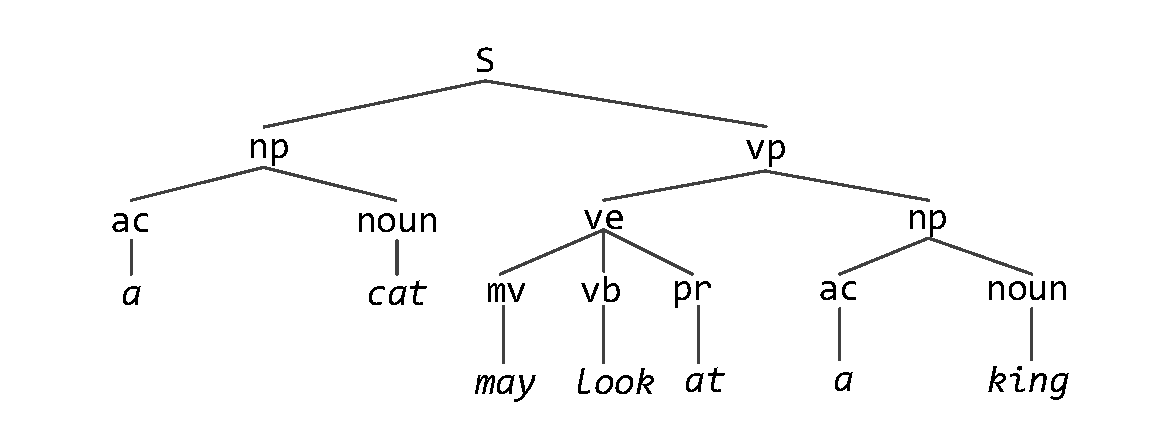
\includegraphics[scale=0.65]{gramtree}
	\end{figure}
	
\end{frame}


\begin{frame}
	\frametitle{\insertsection}
	
	\begin{itemize}
		\item A string of non-terminal symbols (words) is \textbf{grammatically correct} according to our grammar if we can build a parse tree for it. Having a grammar like one above we can
		implement \textbf{a recognizer}~--- a program that correctly classifies strings as being grammatical or not.
		\item In addition to knowing whether a string is grammatical or not, we are interested in why it is grammatical. More precisely, we often want to know what its structure is, and this is exactly the information a parse tree gives us. This kind of information would be important if we were using this sentence in some application and needed to say what it actually meant.
		A program that correctly answers if a string is grammatical and also builds a parse tree is called \textbf{a parser}.
	\end{itemize}
\end{frame}


\begin{frame}
	\frametitle{\insertsection}
	
	\begin{itemize}
		\item A context free language is a language that can be generated by a context free grammar.
		\item It is proved that some natural languages are context free (for example English and French).
		\item Many programming languages are context free languages.
		\item For this reason context free grammars are often used in compiler development.
	\end{itemize}
\end{frame}


\section{DCG in Prolog}

\begin{frame}
	\frametitle{\insertsection}
	
	Let us put it in practice.
	
	\texttt{\begin{tabular}{l}
			sentense(S) :- nounPhrase(NP), verbPhrase(VP), append(NP,VP,S).\\
			nounPhrase(NP) :- article(A), noun(N), append(A,N,NP).\\
			verbPhrase(VP) :- verbExpr(VE), nounPhrase(NP), append(VE,NP,VP).\\
			verbExpr(VE) :- modalVerb(MV),verb(V),prep(P),append([MV,V,P],VE).\\
			article([A]) :- lexicon(''article'', A).\\
			noun([N]) :- lexicon(''noun'',N).\\
			modalVerb([MV]) :- lexicon(''modal verb'',MV).\\
			verb([V]) :- lexicon(''verb'',V).\\
			prep([P]) :- lexicon(''prep'',P).
	\end{tabular}}
\end{frame}


\begin{frame}
	\frametitle{\insertsection}
	
	Predicate \texttt{lexicon/2} is used to define an alphabet (a set of terminal symbols).
	
	\texttt{\begin{tabular}{l}
			lexicon(''article``,''a``).\\
			lexicon(''article``,''the``).\\
			lexicon(''noun``,''cat``).\\
			lexicon(''noun``,''king``).\\
			lexicon(''verb``,''look``).\\
			lexicon(''modal verb``,''may``).\\
			lexicon(''prep``,''at``).
	\end{tabular}}
\end{frame}


\begin{frame}
	\frametitle{\insertsection}
	
	Then add two predicates that are handy when you start a program. Predicate \texttt{recognize} asks user to input string and starts recognizer, \texttt{generate} starts language generator that returns all phrases that are grammatically correct according to grammar.
	\texttt{\begin{itemize}
			\item[] recognize :- write(''Enter the phrase: ''),\\
			\quad\quad\quad\quad\quad\quad\quad current\_input(In),\\
			\quad\quad\quad\quad\quad\quad\quad read\_string(In, ''\textbackslash n'', ''\textbackslash r\textbackslash t'', \_, Phrase),\\
			\quad\quad\quad\quad\quad\quad\quad split\_string(Phrase,~"~",~"",~ListPhrase),\\
			\quad\quad\quad\quad\quad\quad\quad sentense(ListPhrase),!.
			\item[] generate :- sentense(Phrase),\\
			\quad\quad\quad\quad\quad\quad\quad atomics\_to\_string(Phrase,'~',String),\\
			\quad\quad\quad\quad\quad\quad\quad write(String).
	\end{itemize}}
\end{frame}


\begin{frame}
	\frametitle{\insertsection}
	
	This program works, but it is not effective.
	
	\begin{itemize}
		\item The program tries to "guess" parts of a phrase and then afterwards checks whether these can be combined to form the sentence.		
		\item Posing a query \texttt{sentense([''a'',''cat'',''may'',''look'',''at'',''a'',''king''])} will cause the program to check all possible sentences until one of them match the required one.
		\item The problem obviously is, that the goals are called with uninstantiated variables as arguments.
	\end{itemize}
\end{frame}


\begin{frame}
	\frametitle{\insertsection}
	
	We could try and solve the third problem by changing the rules in such a way that \texttt{append} becomes the first goal, but still our program would remain highly ineffective. 
	
	More to it, if we place \texttt{append} to the front generation rules will break.
	
	\texttt{\begin{tabular}{l}
			sentense(S) :- append(NP,VP,S), nounPhrase(NP), verbPhrase(VP).\\
			nounPhrase(NP) :- append(A,N,NP), article(A), noun(N).\\
			verbPhrase(VP) :- append(VE,NP,VP), verbExpr(VE), nounPhrase(NP).\\
			verbExpr(VE) :- append([MV,V,P],VE),\\
			\quad\quad\quad\quad\quad\quad\quad\quad modalVerb(MV),\\
			\quad\quad\quad\quad\quad\quad\quad\quad verb(V),\\
			\quad\quad\quad\quad\quad\quad\quad\quad prep(P).
	\end{tabular}}
\end{frame}


\section{Recognition using difference lists}


\begin{frame}
	\frametitle{\insertsection}
	
	Consider:
	
	\begin{tabular}{m{7cm} m{6cm}}
			\texttt{Ls = [x, y, z| Rs]}. & \% \texttt{Ls} is a partial list, because \texttt{Rs} is uninstantiated \\
			\uncover<2->{
				 \textbf{Symbolically}: \(Ls = [x, y, z] + Rs\) & \(\Leftrightarrow \) \texttt{append([x, y, z], Rs, Ls)} \\
			 }
			\uncover<3->{\textbf{Symbolically}: \(Ls - Rs = [x, y, z]\) & \texttt{[x, y, z]} is the \textbf{list difference} between \texttt{Ls} and \texttt{Rs} \\}
			\uncover<4->{\texttt{Rs = [].} & \texttt{Ls = [x, y, z]} \\}
			\uncover<4->{\texttt{Rs = [a, b]} & \texttt{Ls = [x, y, z, a, b]} \\}
			\uncover<5->{\texttt{Ls0 = [x, y| Ls1], Ls1 = [z, k| Ls2], Ls2 = [...| Ls3]} & An efficient concatenation \\}
			\uncover<6->{\(D_0 = Ls0 - Ls1, D_1 = Ls1 - Ls2, D_2 = Ls2 = Ls3 \) & \(D_0 + D_1 + D_2 = Ls0 - Ls3 \)}
	\end{tabular}
\end{frame}


\begin{frame}
	\frametitle{\insertsection}
	
	The pair of lists \texttt{S} and \texttt{D} represents a sentence if \((a) \) We can consume \texttt{S} and leave behind a \texttt{VP}, and the pair \texttt{S} and \texttt{VP} represents a noun phrase, and	\((b) \) We can then go on to consume \texttt{VP} leaving \texttt{D} behind, and the pair \texttt{VP, D} represents a verb phrase.
	That is: the sentence we are interested in is the difference between the contents of the two lists.
	
	\texttt{\begin{tabular}{l}
			sentense(S,D) :- nounPhrase(S,VP), verbPhrase(VP,D).\\
			nounPhrase(NP,D) :- article(NP,N), noun(N,D).\\
			verbPhrase(VP,D) :- verbExpr(VP,VE), nounPhrase(VE,D).\\
			verbExpr(VE,D) :- modalVerb(VE,MV), verb(MV,V), prep(V,D).\\
			article([A|D],D) :- lexicon(''article'',A).\\
			noun([N|D],D) :- lexicon(''noun'',N).\\
			modalVerb([MV|D],D) :- lexicon(''modal verb'',MV).\\
			verb([V|D],D) :- lexicon(''verb'',V).\\
			prep([P|D],D) :- lexicon(''prep'',P).\\
	\end{tabular}}
\end{frame}


\begin{frame}
	\frametitle{\insertsection}
	
	DCGs are really ``syntactic sugar'' for grammars written in terms of difference lists.
	
	\texttt{\begin{tabular}{l}
			sentense -{}-\textgreater~nounPhrase, verbPhrase.\\
			nounPhrase -{}-\textgreater~article, noun.\\
			verbPhrase -{}-\textgreater~verbExpr, nounPhrase.\\
			verbExpr -{}-\textgreater~modalVerb, verb, prep.\\
			article -{}-\textgreater~[''a''].\\
			article -{}-\textgreater~[''the''].\\
			noun -{}-\textgreater~[''cat''].\\
			noun -{}-\textgreater~[''king''].\\
			modalVerb -{}-\textgreater~[''may''].\\
			verb -{}-\textgreater~[''look''].\\
			prep -{}-\textgreater~[''at''].\\
	\end{tabular}}
\end{frame}


\section{Recursive rules}


\begin{frame}
	\frametitle{\insertsection}
	
	Suppose we want to add a conjunctive rule to our little grammar:
	
	\begin{table}
		\centering
		\begin{tabular}{ l }
			\rowcolor{LightGray} sentense \(\rightarrow \) sentense conjunction sentense \\
			\rowcolor{LightGray} conjunction \(\rightarrow \) and \\
			\rowcolor{LightGray} conjunction \(\rightarrow \) or \\
			\rowcolor{LightGray} conjunction \(\rightarrow \) but \\
		\end{tabular}
	\end{table}
\end{frame}


\begin{frame}
	\frametitle{\insertsection}
	
	A piece of cake, isn't it?
	
	\texttt{\begin{tabular}{l}
			sentense -{}-\textgreater~sentense, conjunction, sentense.\\
			conjunction -{}-\textgreater~[''and''].\\
			conjunction -{}-\textgreater~[''or''].\\
			conjunction -{}-\textgreater~[''but''].\\
	\end{tabular}}

	Nice try, but no...
\end{frame}


\begin{frame}
	\frametitle{\insertsection}
	
	If we place the recursive rule before the non-recursive rule
	
	\texttt{sentense -{}-\textgreater~nounPhrase, verbPhrase}
	
	then the knowledge base will contain the following two Prolog rules, in this order:
	
	\texttt{\begin{table}
			\centering
			\begin{tabular}{l}
				sentence(A, B) :- sentence(A, C), conjunction(C, D), sentence(D, B).\\
				sentence(A, B) :- nounPhrase(A, C), verbPhrase(C, B).
			\end{tabular}
	\end{table}}

	When Prolog tries to use the first rule, it immediately encounters the recursive goal, which it then tries to satisfy using the first rule, whereupon it immediately encounters the same goal and so on infinitely... Prolog goes into infinite loop and does no useful work.
	
\end{frame}


\begin{frame}
	\frametitle{\insertsection}
	
	So, let us add the recursive rule at the end of the knowledge base making Prolog always encounter the non-recursive rule first. 
	
	What happens now when we try to recognize grammatically correct sentence? Prolog seems to be able to handle it and gives the right answer. But when we pose an ungrammatical sentence, Prolog again gets into an infinite loop. 
	
	Since it is unable to recognize our sentence as consisting of a noun phrase and a verb phrase, Prolog tries to analyze it with a recursive rule again and again, and ends up in the same loop as before.
	
	\texttt{
			\begin{tabular}{l l}
				?- sentence(["a", "cat", "may", "look", "at", "the", "king"], []) & true.\\
				?- sentence(["a", "cat"], []). & ERROR
			\end{tabular}
	}
	
\end{frame}


\begin{frame}
	\frametitle{\insertsection}
	
	Recall, that in the case of ordinary recursive rule (not DCG) the trick was to change goals of the recursive rule so that the recursive goal is not the first one in the body of the rule.
	
	In the case of DCG this is not a solution, since the order of the goals determines the order of the words in the sentence.
	
	\texttt{\begin{tabular}{m{15cm}}
			sentence(A, B) :- sentence(A, C), conjunction(C, D), sentence(D, B). \(\nLeftrightarrow \) sentence(A, B) :- conjunction(C, D), sentence(A, C), sentence(D, B).
	\end{tabular}}
	
\end{frame}


\begin{frame}
	\frametitle{\insertsection}
	
	What do we do then? The only possible solution we have is to introduce new non-terminal symbols.
	
	\texttt{\begin{table}
			\centering
			\begin{tabular}{l}
				plainSentense -{}-\textgreater~nounPhrase, verbPhrase.\\
				sentense -{}-\textgreater~plainSentense.\\
				sentense -{}-\textgreater~plainSentense, conjunction, sentense.\\
			\end{tabular}
	\end{table}}
	
\end{frame}


\section{Formal languages}

\begin{frame}
	\frametitle{\insertsection}
	
	A simple example of a formal language is \(a^nb^n\). There are only two ''words`` in this language: the symbol \(a\) and the symbol \(b\).
	The language \(a^nb^n\) consist of all strings made up from these two symbols that have the following form: the string must consist of an unbroken block of \(a\)s of length \(n\), followed by an unbroken block of \(b\)s of length \(n\), and nothing else. Note that the empty word \(\mathcal{E} \) also belongs to \(a^nb^n \).
	
	\uncover<2->{\texttt{\begin{table}
				\centering
				\begin{tabular}{l}
					s --> [].\\
					s --> [a],s,[b].
				\end{tabular}
	\end{table}}}
	
\end{frame}



% Lesson 9. Definite Clause Grammars. Continue.
\lecture{DCG}{dcgc}

\section{Overview}

\begin{frame}
	\frametitle{\insertsection}
	Goals of the lesson
	\begin{itemize}
		\item To examine extra arguments and extra tests offered by DCG notation.
		\item To discuss the limitations of DCGs.
	\end{itemize}
\end{frame}


\section{Extra arguments}

\begin{frame}
	\frametitle{\insertsection}
	
	Recall the grammar we built on the previous class:
	
	\begin{table}
		\centering
		\begin{tabular}{ l }
			\rowcolor{LightGray} S \(\rightarrow \) nounPhrase verbPhrase \\
			\rowcolor{LightGray} nounPhrase \(\rightarrow \) article noun \\
			\rowcolor{LightGray} verbPhrase \(\rightarrow \) verbExpr nounPhrase \\
			\rowcolor{LightGray} verbExpr \(\rightarrow \) modalVerb verb prep \\
			\rowcolor{LightGray} article \(\rightarrow \) a \\
			\rowcolor{LightGray} article \(\rightarrow \) the \\
			\rowcolor{LightGray} noun \(\rightarrow \) cat \\
			\rowcolor{LightGray} noun \(\rightarrow \) king \\
			\rowcolor{LightGray} modalVerb \(\rightarrow \) may \\
			\rowcolor{LightGray} verb \(\rightarrow \) look \\
			\rowcolor{LightGray} prep \(\rightarrow \) at
		\end{tabular}
	\end{table}

\end{frame}


\begin{frame}
	\frametitle{\insertsection}
	
	As we know this grammar produces sentences like:
	
	\begin{itemize}
		\item A cat may look at a king
		\item A cat may look at the king
		\item A king may look at a cat
		\item A king may look at the cat
		\item The cat may look at a king
		\item The king may look at a cat
	\end{itemize}

	And so on, around 20 sentences in total.
\end{frame}


\begin{frame}
	\frametitle{\insertsection}
	
	Suppose we wanted to add pronouns, and deal with sentences like:
	
	\begin{itemize}
		\item He may look at her
		\item A cat may look at him
		\item A king may look at her
		\item She may look at a cat
	\end{itemize}

	There are subjective and objective pronouns.
\end{frame}


\begin{frame}
	\frametitle{\insertsection}
	
	Hmm, nice, let us add rules for pronouns:
	
	\texttt{\begin{table}
			\centering
			\begin{tabular}{l}
				pro -{}-\textgreater ["he"].\\
				pro -{}-\textgreater ["him"].\\
				pro -{}-\textgreater ["she"].\\
				pro -{}-\textgreater ["her"].\\
				nounPhrase -{}-\textgreater pro.
			\end{tabular}
	\end{table}}
\end{frame}


\begin{frame}
	\frametitle{\insertsection}
	
	Up to a point this grammar works. It recognizes and generates all sentences we wanted it to, but it will also accept a lot of sentences that are clearly wrong.
	
	\begin{itemize}
		\item Him may look at a cat
		\item He may look at she
		\item The king may look at she
		\item The cat may look at she
	\end{itemize}
	
\end{frame}


\begin{frame}
	\frametitle{\insertsection}

	Definite Clause Grammar is just a language model. It possesses no knowledge about English phrases. 
	
	That is, accepting a sentence \textit{''A cat may look at she``} it doesn’t know that “she” and “he” are subject pronouns and cannot be used in object position.
	
	Moreover, accepting \textit{''Him may look at a cat``} it doesn't know either that “her” and “him” are object pronouns and cannot be used in subject position.
	
\end{frame}


\begin{frame}
	\frametitle{\insertsection}
	
	\begin{table}
		\centering
		\begin{tabular}{| c | c | c | c | c |}
			\hline
			\multirow{2}{*}{\textbf{PERSONS}} & \multicolumn{2}{|c|}{\textbf{SINGULAR}} & \multicolumn{2}{|c|}{\textbf{PLURAL}} \\ \cline{2-5}
			& \textbf{Subjective Case} & \textbf{Objective Case} & \textbf{Subjective Case} & \textbf{Objective Case} \\
			\hline
			\textbf{\(1^{st}\) person} & I & me & we & us \\
			\hline
			\textbf{\(2^{nd}\) person} & you & you & you & you \\
			\hline
			\textbf{\(3^{rd}\) person} & he,she,it & him,her,it & they & them \\
			\hline
		\end{tabular}
	\end{table}
\end{frame}


\begin{frame}
	\frametitle{\insertsection}
	
	Now it is obvious that we have to explicitly state which pronoun can and which cannot occur in a subject position.
	\texttt{\begin{table}
			\centering
			\begin{tabular}{l}
				sentense -{}-\textgreater ~subjNP, verbPhrase.\\
				subjNP -{}-\textgreater ~article, noun.\\
				subjNP -{}-\textgreater ~spr.\\
				objNP -{}-\textgreater ~article, noun.\\
				objNP -{}-\textgreater ~opr.\\
				verbPhrase -{}-\textgreater ~verbExpr, objNP.\\
				spr -{}-\textgreater ~~["he"]. \\
				spr -{}-\textgreater ~["she"]. \\
				opr -{}-\textgreater ~["him"]. \\
				opr -{}-\textgreater ~["her"]. \\
			\end{tabular}
	\end{table}}
	
\end{frame}


\begin{frame}
	\frametitle{\insertsection}
	
	It works now. This solution, however, cannot be considered a good one.
	
	A small addition to the lexicon has led to quite a big change in the grammar. In particular, we’ve doubled the number of noun phrase rules.
	
	If we wanted to make more changes, let's say it to further extend the lexicon, things would get even worse.
	
\end{frame}


\begin{frame}
	\frametitle{\insertsection}
	
	What we truly need is some elegant programming technique, and here is where the extra arguments come into play.
	
	\textbf{Consider the following program:}
	\texttt{\begin{table}
			\centering
			\begin{tabular}{l l}
				sentense -{}-\textgreater~ nounPhrase(subj),verbPhrase. & article -{}-\textgreater~ ["a"]. \\
				nounPhrase(\_) -{}-\textgreater~ article, noun. & article -{}-\textgreater~ ["the"]. \\
				nounPhrase(P) -{}-\textgreater~ pro(P). & noun -{}-\textgreater~ ["cat"]. \\
				verbPhrase -{}-\textgreater~ verbExpr, nounPhrase(obj). & noun -{}-\textgreater~ ["king"]. \\
				verbExpr -{}-\textgreater~ modalVerb, verb, prep. & pro(subj) -{}-\textgreater~ ["he"]. \\
				modalVerb -{}-\textgreater~ ["may"]. & pro(subj) -{}-\textgreater~ ["she"]. \\
				verb -{}-\textgreater~ ["look"]. & pro(obj) -{}-\textgreater~ ["him"]. \\
				prep -{}-\textgreater~ ["at"]. & pro(obj) --> ["her"].
			\end{tabular}
	\end{table}}
	
\end{frame}


\begin{frame}
	\frametitle{\insertsection}
	
	We already know (or at least I hope we do) that any DCG rule is just a syntactic sugar for an ordinary Prolog rule. So, what \texttt{sentence -{}-\textgreater~ nounPhrase(subj)} translates into?
	\texttt{\begin{table}
			\centering
			\begin{tabular}{l}
				 ~sentense -{}-\textgreater~ nounPhrase,verbPhrase.\\
				 ~sentense(A,B) :- nounPhrase(A,C),verbPhrase(C,B).\\ \\
				\hline \hline
				\\
				\uncover<2->{
					sentense -{}-\textgreater~ nounPhrase(subj),verbPhrase.\\
					~sentense(A,B) :- nounPhrase(subj,A,C),verbPhrase(C,B).
				}
			\end{tabular}
	\end{table}}
	
\end{frame}


\begin{frame}
	\frametitle{\insertsection}
	
	One final remark: don’t be misled by this simplicity of our example. Extra arguments can be used to cope with some complex syntactic problems. 
	
	DCGs are no longer the state-of-art grammar development tools they once were, but they’re not toys either. 
	
	Once you know about writing DCGs with extra arguments, you can write some fairly sophisticated grammars.
\end{frame}


\section{Making parsers}

\begin{frame}
	\frametitle{\insertsection}
	
	So far, our programs have been able to answer \textit{''yes``} or \textit{''no``} whether the input sentence correct according to the grammar, and produce grammatical output.
	
	That is, they all were \textit{recognizers}.
	
	But what if we would like them to not only tell us which sentences are grammatical, but also to analyze their structures. For example we would like to see the parse trees.
	
\end{frame}


\begin{frame}
	\frametitle{\insertsection}
	
	Considering the tree:
	
	\begin{figure}
		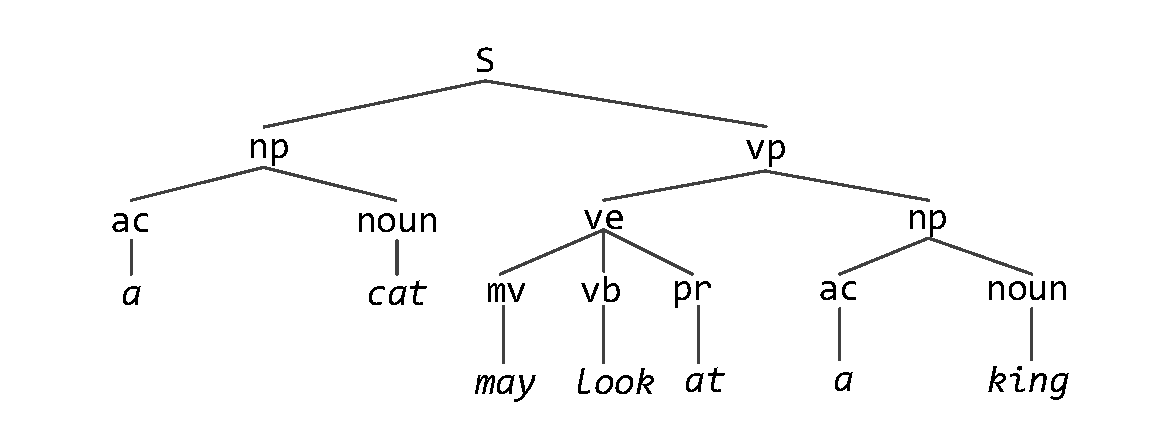
\includegraphics[scale=0.65]{gramtree}
	\end{figure}
\end{frame}


\begin{frame}
	\frametitle{\insertsection}
	
	We could make a following DCG:

	\texttt{\begin{tabular}{l}
			sentense(s(NP,VP)) -{}-\textgreater~ nounPhrase(NP), verbPhrase(VP).\\
			nounPhrase(np(A,N)) -{}-\textgreater~ article(A), noun(N).\\
			verbPhrase(vp(VE,NP)) -{}-\textgreater~ verbExpr(VE), nounPhrase(NP).\\
			verbExpr(ve(MV,V,P)) -{}-\textgreater~ modalVerb(MV), verb(V), prep(P).\\
			article(art("a")) -{}-\textgreater~ ["a"].\\
			article(art("the")) -{}-\textgreater~ ["the"].\\
			noun(n("cat")) -{}-\textgreater~ ["cat"].\\
			noun(n("king")) -{}-\textgreater~ ["king"].\\
			modalVerb(mv("may")) -{}-\textgreater~ ["may"].\\
			verb(v("look")) -{}-\textgreater~ ["look"].\\
			prep(p("at")) -{}-\textgreater~ ["at"].\\
	\end{tabular}}
	
\end{frame}


\begin{frame}
	\frametitle{\insertsection}
	
	Corresponding to our proverb we could have the following result:
	\texttt{\begin{table}
			\centering
			\begin{tabular}{m{14cm}}
				?- sentence(T, [''a``, ''cat``, ''may``, ''look``, ''at``, ''a``, ''king''], []). \\ \\
				T = s(np(art(''a``), n(''cat``)), vp(ve(mv(''may``), v(''look``), p(''at``)), np(art(''a``), n(''king``)))).\\
			\end{tabular}
	\end{table}}


	It may not look nice, but it contains all the information from the picture. Depending on the task, we can design the output to our liking.
	
\end{frame}



\section{Extra goals}

\begin{frame}
	\frametitle{\insertsection}
	
	When haven't used DCG notations we introduced a special predicate \texttt{lexicon/2} to define our alphabet.
	
	\only<1>{\texttt{\begin{tabular}{l}
			sentense(S,D) :- nounPhrase(S,VP), verbPhrase(VP,D).\\
			nounPhrase(NP,D) :- article(NP,N), noun(N,D).\\
			verbPhrase(VP,D) :- verbExpr(VP,VE), nounPhrase(VE,D).\\
			verbExpr(VE,D) :- modalVerb(VE,MV), verb(MV,V), prep(V,D).\\
			article([A|D],D) :- lexicon(''article'',A).\\
			noun([N|D],D) :- lexicon(''noun'',N).\\
			modalVerb([MV|D],D) :- lexicon(''modal verb'',MV).\\
			verb([V|D],D) :- lexicon(''verb'',V).\\
			prep([P|D],D) :- lexicon(''prep'',P).\\
	\end{tabular}}}
	
	\only<2->{\texttt{\begin{tabular}{l}
				lexicon(''article``,''a``).\\
				lexicon(''article``,''the``).\\
				lexicon(''noun``,''cat``).\\
				lexicon(''noun``,''king``).\\
				lexicon(''verb``,''look``).\\
				lexicon(''modal verb``,''may``).\\
				lexicon(''prep``,''at``).
	\end{tabular}}}

	\only<3->{Why haven't we done the same thing in DCG notation then? \textbf{Is it possible?}}
	
\end{frame}


\begin{frame}
	\frametitle{\insertsection}
	
	Why, of cause it is!
	
	\texttt{\begin{tabular}{l}
			sentense -{}-\textgreater~nounPhrase, verbPhrase.\\
			nounPhrase -{}-\textgreater~article, noun.\\
			verbPhrase -{}-\textgreater~verbExpr, nounPhrase.\\
			verbExpr -{}-\textgreater~modalVerb, verb, prep.\\ \\
			article -{}-\textgreater~\{lexicon("article",A)\},[A].\\
			noun -{}-\textgreater~\{lexicon("noun",Noun)\},[Noun].\\
			modalVerb -{}-\textgreater~\{lexicon("modal verb",Mv)\},[Mv].\\
			verb -{}-\textgreater~\{lexicon("verb",Verb)\},[Verb].\\
			prep -{}-\textgreater~\{lexicon("prep",Prep)\},[Prep].\\
	\end{tabular}}
	
\end{frame}


\begin{frame}
	\frametitle{\insertsection}
	
	The extra goals can be written anywhere on the right side of a DCG rule, but \textbf{must stand between curly brackets}. When Prolog encounters such curly brackets while translating a DCG into its internal representation, it just takes the extra goals specified between the curly brackets over into the translation.
	
	The extra arguments give us the tools for coping with any computable language whatsoever, not just context free languages.
	
	For example, the formal language \(a^nb^nc^n-\{\varepsilon \}\) is not a context free language. It could be proved by contradiction that you will not succeed in writing a context free grammar that generates precisely these strings.
		
\end{frame}


\begin{frame}
	\frametitle{\insertsection}
	
	What we need to make a DCG for \(a^nb^nc^n-\{\varepsilon \}\) is a symbol counter. Any correct string has to have a block of \(a\)s followed by a block of \(b\)s followed by a block of \(c\)s, and all blocks are to have the same length.
	
	\texttt{\begin{tabular}{l}
			as(0) -{}-\textgreater~ [].\\
			as(Len) -{}-\textgreater~ [a],as(Prev), \{Len is Prev + 1\}.\\
			bs(0) -{}-\textgreater~ [].\\
			bs(Len) -{}-\textgreater~ [b],bs(Prev), \{Len is Prev + 1\}.\\
			cs(0) -{}-\textgreater~ [].\\
			cs(Len) -{}-\textgreater~ [c],cs(Prev), \{Len is Prev + 1\}.\\
	\end{tabular}}
\end{frame}


\begin{frame}
	\frametitle{\insertsection}
	
	The second rule for the non-terminal \texttt{as} would be translated as follows:
	
	\texttt{\begin{table}\centering\begin{tabular}{l}
			as(Len,A,B) :- ’C’(A, a, C), \\ \quad\quad\quad\quad\quad\quad\quad\quad
			as(Prev, C, B), \\ \quad\quad\quad\quad\quad\quad\quad\quad
			Len is Prev + 1.
	\end{tabular}\end{table}}
	
\end{frame}


\section{Conclusions}

\begin{frame}[shrink=7]
	\frametitle{\insertsection}
	
	For the most part, DCGs are presented as a simple tool for developing context free grammars. But as we saw it was possible to extend beyond that. DCGs are programming language in their own right. They are Turing complete.
	
	But they have rather significant drawbacks. They are tendent to loop when goal ordering is wrong. If we need to use lots of extra arguments, they become a rather clumsy mechanism. Many of this problems, however, DCG notation inherits from the Prolog itself. It is well-known that all top-down parsers loop on left-recursive grammars.
	
	DCGs as we saw them, are a nice notation for context free grammars enhanced with some features that comes with a free parser/recognizer, are probably best viewed as a convenient tool for testing new grammatical ideas, or for implementing reasonably complex grammars for particular applications.
	
	With a conventional programming language (such as C++ or Java) it simply wouldn’t be possible to reach this stage so soon. Things would be easier in functional languages (such as LISP, SML, or Haskell), but even so, it is doubtful whether beginners could do so much so early.
\end{frame}


% Lesson 10. Advanced in terms
\lecture{TADV}{tadv}


\section{Overview}

\begin{frame}
	\frametitle{\insertsection}
	
	Goals of the lesson
	\begin{itemize}
		\item To introduce operators
		\item To recall term comparison operators
		\item To discuss term decomposition operations
	\end{itemize}
	
\end{frame}


\section{Comparison}

\begin{frame}
	\frametitle{\insertsection}
	
	\begin{tabular}{m{14cm}}
		Prolog contains an important predicate for comparing terms, namely \texttt{==/2}. It \textbf{does not instantiate} variables, thus it is not the same as the unification predicate \texttt{=/2}.\\ \\
		\texttt{term1 == term2} is \texttt{true} if and only if \texttt{term1} and \texttt{term2} are identical.
		\only<5->{\\ \\ It should now be clear that \texttt{==} can be viewed as a \textit{\textbf{stronger}} test for equality between terms than \texttt{=}. That is, if \texttt{t1} and \texttt{t2} are Prolog terms, and the query \texttt{t1 == t2} succeeds, then the query \texttt{t1 = t2} will succeed too.}
	\end{tabular}
	
	\only<2>{\texttt{
		\begin{table}
			\centering
			\begin{tabular}{l l}
				term == term. & true.\\ \\
				term1 == term2. & false.\\ \\
				term == 'term'. & true.
			\end{tabular}
		\end{table}
	}}

	\only<3-4>{\texttt{
			\begin{table}
				\centering
				\begin{tabular}{l l}
					X == Y. & \uncover<4>{false.}\\ \\
					X == a. & \uncover<4>{false.}\\ \\
					X = a, X == a. & \uncover<4>{true.}\\ \\
					X = Y, X == Y. & \uncover<4>{true.}
				\end{tabular}
			\end{table}
	}}

	
\end{frame}


\begin{frame}
	\frametitle{\insertsection}
	
	A predicate that is reverse of \texttt{==} is \texttt{\textbackslash==}. This predicate id defined so that it succeeds precisely in those case where \texttt{==} fails.
	
	\texttt{\begin{table}
			\centering
			\begin{tabular}{l l}
				term \textbackslash== term. & \uncover<2->{false.}\\ \\
				t1 \textbackslash== t2. & \uncover<2->{true.}\\ \\
				term \textbackslash== 'term'. & \uncover<2->{false.}\\ \\
				X \textbackslash== a. & \uncover<2->{true.}\\ \\
				X \textbackslash== Y. & \uncover<2->{true.}
			\end{tabular}
	\end{table}}
\end{frame}


\begin{frame}
	\frametitle{\insertsection}
	
	Now we have introduced all comparing terms. Here is the summary:
	
	\begin{table}
		\centering
		\begin{tabular}{l m{10cm}}
			\rowcolor{LightGray} = & The unification predicate. Succeeds if it can unify its arguments, fails otherwise.\\
			\rowcolor{LightGray} \textbackslash= & The negation of the unification predicate. Succeeds if = fails, and vice-versa.\\
			\rowcolor{LightGray} == & The identity predicate. Succeeds if its arguments are identical, fails otherwise.\\
			\rowcolor{LightGray} \textbackslash== & The negation of the identity predicate. Succeeds if == fails, and vice-versa.\\
			\rowcolor{LightGray} =:= & The arithmetic equality predicate. Succeeds if its arguments evaluate to the same integer.\\
			\rowcolor{LightGray} =\textbackslash= & The arithmetic inequality predicate. Succeeds if its arguments evaluate to different integers.
		\end{tabular}
	\end{table}
\end{frame}


\section{Term notation}

\begin{frame}
	\frametitle{\insertsection}
	
	Some terms may have multiple notations, and, although they look different to us, Prolog regards them as identical. As we recall, \texttt{t} and \texttt{'t'} are identical, that is these are two different notations of the same term, as far as Prolog is concerned.
	
	In fact there are many other cases there Prolog treats two strings as being exactly the same term. Most of them are \textit{syntactic sugar} that makes programming more pleasant.
	
	It is very handy to be able to write code in the notation we like, and to let Prolog run our code in the notation it finds natural.
\end{frame}


\begin{frame}
	\frametitle{\insertsection}
	
	A good and most obvious example of this are the arithmetic predicates. As we recall, arithmetic operations are terms, having multiple notations.
	
	\only<1>{\texttt{\begin{table}
				\centering
				\begin{tabular}{l c l}
					2 + 3 & == & +(2,3).\\
					2 - 3 & == & -(2,3).\\
					2 * 3 & == & *(2,3).\\
					3 * (7 + 5) & == & *(3, +(7,5)).
				\end{tabular}
			\end{table}}}

	\only<2->{\texttt{\begin{table}
				\centering
				\begin{tabular}{l c l}
					(2 < 3) & == & <(2, 3).\\
					(2 =< 3) & == & =<(2, 3).\\
					(2 =:= 3) & == & =:=(2, 3).\\
					(2 =\textbackslash= 3) & == & =\textbackslash=(2, 3).\\
					(2 > 3) & == & >(2, 3).\\
					(2 >= 3) & == & >=(2, 3).
				\end{tabular}
			\end{table}}}
	
\end{frame}


\section{Examining terms}

\begin{frame}
	\frametitle{\insertsection}
	
	\begin{figure}
		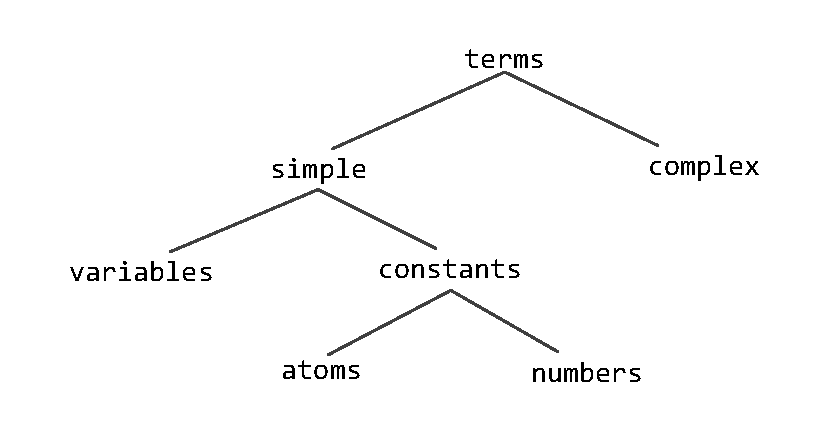
\includegraphics[scale=0.9]{typetree}
	\end{figure}
\end{frame}


\begin{frame}
	\frametitle{\insertsection}
	
	Sometimes it is useful to know of which type a given term is. Prolog provides built-in predicates that test if a given term is of certain type or not.
	
	\begin{table}
		\centering
		\begin{tabular}{ l l }
			\rowcolor{LightGray} \texttt{atom/1} & Tests whether the argument is an atom. \\
			\rowcolor{LightGray} \texttt{integer/1} & Tests whether the argument is an integer. \\
			\rowcolor{LightGray} \texttt{float/1} & Tests whether the argument is a floating point number. \\
			\rowcolor{LightGray} \texttt{number/1} & Tests whether the argument is a number, i.e. an integer or a float. \\
			\rowcolor{LightGray} \texttt{atomic/1} & Tests whether the argument is a constant. \\
			\rowcolor{LightGray} \texttt{var/1} & Tests whether the argument is an uninstantiated variable. \\
			\rowcolor{LightGray} \texttt{nonvar/1} & Tests whether the argument is not an  uninstantiated variable.
		\end{tabular}
	\end{table}
\end{frame}


\begin{frame}
	\frametitle{\insertsection}
	
	Suppose we have a complex term of which we don't know what it looks like. What do we want to know about it?
	
	Probably, what its functor is, what's the arity and what do arguments look like.
	
	Prolog provides built-in predicates that do precisely that.
\end{frame}


\begin{frame}
	\frametitle{\insertsection}
	
	The first two questions are answered by the predicate \texttt{functor/3}. Given a term this predicate will tell us what the functor and the arity are.
	
	\texttt{\begin{tabular}{l l}
			?- functor(f(x, y), F, A). & F = f, A = 2.\\ \\
			?- functor(f, F, A). & F = f, A = 0.
	\end{tabular}}

	We can use the predicate \texttt{functor/3} not only to find the structure of a term, but also to \textbf{construct} terms. How? By specifying the second and third arguments and leaving the first uninstantiated.
	
	\texttt{\begin{tabular}{l l}
			?- functor(T, f, 3). & T = f(\_21882, \_21884, \_21886).
	\end{tabular}}
	
	\textbf{Note, that either the first argument or the second and third argument have to be instantiated.}
\end{frame}


\begin{frame}
	\frametitle{\insertsection}
	
	The third question about the structure of an unknown complex term is answered by two predicates.
	
	The first is \texttt{arg/3} which tells us about arguments of complex term. It takes a number \(N \) and a term \texttt{T} and returns the \(N\)-th argument of \texttt{T} as its last argument. It can be used either to access the value or to instantiate a corresponding argument.
	
	\texttt{\begin{tabular}{l l}
			?- arg(2, f(x, y), Second). & Second = y.\\
			?- arg(2, f(x, Y), y). & Y = y.\\
			?- arg(3, f(x, y), Third). & false.
	\end{tabular}}

	\textbf{Note that enumeration on arguments starts at 1.}
\end{frame}


\begin{frame}
	\frametitle{\insertsection}
	
	The second is \texttt{'=..'/2}. It takes a complex term and returns a list containing the functor as first element and then all the arguments. This predicate is called \textbf{univ}.
	
	\texttt{\begin{tabular}{l l}
			?- f(x, y, z) =.. Struct. & Struct = [f, x, y, z].\\
			?- f(X) =.. F. & F = [f, X].\\
			?- T =.. [g, x, y, z]. & T = g(x, y, z).
	\end{tabular}}
\end{frame}


\section{Operators}

\begin{frame}
	\frametitle{\insertsection}
	
	Operators are the unary or binary predicates defined as:
	
	\begin{enumerate}
		\item \textit{Infix} operator. They are written between their arguments.
		\item \textit{Prefix} operator that are written before their argument.
		\item \textit{Postfix} operator which is written after their argument.
	\end{enumerate}
\end{frame}


\begin{frame}
	\frametitle{\insertsection}
	
	Prolog standard predicate notations are not ambiguous. For example we wouldn't be confused on how to interpret the expression \texttt{is(11, +(2, *(3,3)))}, because it is pretty obvious in which order operations should be performed.
	
	Other notations, however, could be more ambiguous. For example Prolog knows about conventions for disambiguating arithmetic expressions. When we write \texttt{2 + 3 * 3}, Prolog knows that it is \texttt{2 + (3 * 3)} we meant, not \texttt{(2 + 3) * 3}.
	
	Such conventions are implemented with operator \textit{precedence}. Every operator has a certain precedence. The precedence of \texttt{+} is greater that the precedence of \texttt{*}, for instance. In the expression \texttt{2 + 3 * 3} operator \texttt{+} has the highest precedence, so it is taken to be the main functor of the expression: \texttt{+(2, *(3,3))}.
	
	The precedence of \texttt{is/2} is higher than the precedence of any arithmetic operator, so that \texttt{11 is 2 + 3 * 3} is interpreted as \texttt{is(11, +(2, *(3, 3))))}.
\end{frame}


\begin{frame}
	\frametitle{\insertsection}
	
	OK, that is what about precedence. Let us look to the following query, though.
	
	\texttt{?- 6 is 1 + 2 + 3.}
	
	Prolog correctly answers \texttt{true}. But how Prolog parenthesizes the internal representation: \texttt{is(6, +(1, +(2, 3)))} or \texttt{is(6, +(+(1, 2), 3))}?
	
	Prolog uses information about the \textbf{associativity} of operations to disambiguate the expressions.
	
	For example, \texttt{+} is \textit{left associative}. That means the expression to the right of + must have a lower precedence that + itself, whereas the expression to the left may have the same precedence as +.
	
	Some operators might be defined to be non-associative which means that both of their arguments must have a lower precedence.
\end{frame}


\begin{frame}
	\frametitle{\insertsection}
	
	The type of an operator (infix, prefix, or postfix), its precedence, and its associativity are the three things that Prolog needs to know to be able to translate the user friendly, but potentially ambiguous operator notation into Prolog’s internal representation.

	New operator definitions in Prolog look like:	
	\texttt{\begin{table}
			\centering
			\begin{tabular}{c}
				:- op(Precedence, Type, Name).
			\end{tabular}
	\end{table}}


	\begin{tabular}{m{9cm} c}
		\uncover<2->{Precedence is a number between 0 and 1200.} \uncover<3->{
			Type is an atom specifying the type and associativity of the operator: f represents the operator while x and y represent its arguments, x stands for 
		an argument which must have a precedence lower than the precedence of f, and y stands for an argument which could have the precedence lower or equal to the 
	precedence of f.} & \uncover<3->{{\texttt{
			\begin{tabular}{l l}
				\rowcolor{LightGray} infix & xfx, xfy, yfx \\
				\rowcolor{LightGray} prefix & fx, fy \\
				\rowcolor{LightGray} postfix & xf, yf \\
			\end{tabular}}}}
	\end{tabular}
\end{frame}


\begin{frame}
	\frametitle{\insertsection}
	
	Here are the definitions for some of the built-in operators. You can see that operators with the same properties can be specified in one statement by giving a list of their names instead of a single name as third argument of op.
	\texttt{\begin{table}
			\centering
			\begin{tabular}{ l }
				\rowcolor{LightGray} :- op(1200, xfx, [:-, -\textgreater]). \\
				\rowcolor{LightGray} :- op(1200, fx, [:-, ?- ]). \\
				\rowcolor{LightGray} :- op(1200, xfy, [;]). \\
				\rowcolor{LightGray} :- op(1000, xfy, [',']). \\
				\rowcolor{LightGray} :- op(700, xfx, [=, is, =.., ==, \textbackslash==, =:=, =\textbackslash=, <, >, =<, >=]). \\
				\rowcolor{LightGray} :- op(500, yfx, [+, -]). \\
				\rowcolor{LightGray} :- op(500, fx, [+, -]). \\
				\rowcolor{LightGray} :- op(300, xfx, [mod]). \\
				\rowcolor{LightGray} :- op(200, xfy, [\textasciicircum]). \\
			\end{tabular}
	\end{table}}
	
\end{frame}
